% Options for packages loaded elsewhere
\PassOptionsToPackage{unicode}{hyperref}
\PassOptionsToPackage{hyphens}{url}
\PassOptionsToPackage{dvipsnames,svgnames,x11names}{xcolor}
%
\documentclass[
  letterpaper,
]{report}

\usepackage{amsmath,amssymb}
\usepackage{iftex}
\ifPDFTeX
  \usepackage[T1]{fontenc}
  \usepackage[utf8]{inputenc}
  \usepackage{textcomp} % provide euro and other symbols
\else % if luatex or xetex
  \usepackage{unicode-math}
  \defaultfontfeatures{Scale=MatchLowercase}
  \defaultfontfeatures[\rmfamily]{Ligatures=TeX,Scale=1}
\fi
\usepackage{lmodern}
\ifPDFTeX\else  
    % xetex/luatex font selection
\fi
% Use upquote if available, for straight quotes in verbatim environments
\IfFileExists{upquote.sty}{\usepackage{upquote}}{}
\IfFileExists{microtype.sty}{% use microtype if available
  \usepackage[]{microtype}
  \UseMicrotypeSet[protrusion]{basicmath} % disable protrusion for tt fonts
}{}
\makeatletter
\@ifundefined{KOMAClassName}{% if non-KOMA class
  \IfFileExists{parskip.sty}{%
    \usepackage{parskip}
  }{% else
    \setlength{\parindent}{0pt}
    \setlength{\parskip}{6pt plus 2pt minus 1pt}}
}{% if KOMA class
  \KOMAoptions{parskip=half}}
\makeatother
\usepackage{xcolor}
\usepackage[top=30mm,left=20mm]{geometry}
\setlength{\emergencystretch}{3em} % prevent overfull lines
\setcounter{secnumdepth}{5}
% Make \paragraph and \subparagraph free-standing
\ifx\paragraph\undefined\else
  \let\oldparagraph\paragraph
  \renewcommand{\paragraph}[1]{\oldparagraph{#1}\mbox{}}
\fi
\ifx\subparagraph\undefined\else
  \let\oldsubparagraph\subparagraph
  \renewcommand{\subparagraph}[1]{\oldsubparagraph{#1}\mbox{}}
\fi

\usepackage{color}
\usepackage{fancyvrb}
\newcommand{\VerbBar}{|}
\newcommand{\VERB}{\Verb[commandchars=\\\{\}]}
\DefineVerbatimEnvironment{Highlighting}{Verbatim}{commandchars=\\\{\}}
% Add ',fontsize=\small' for more characters per line
\usepackage{framed}
\definecolor{shadecolor}{RGB}{241,243,245}
\newenvironment{Shaded}{\begin{snugshade}}{\end{snugshade}}
\newcommand{\AlertTok}[1]{\textcolor[rgb]{0.68,0.00,0.00}{#1}}
\newcommand{\AnnotationTok}[1]{\textcolor[rgb]{0.37,0.37,0.37}{#1}}
\newcommand{\AttributeTok}[1]{\textcolor[rgb]{0.40,0.45,0.13}{#1}}
\newcommand{\BaseNTok}[1]{\textcolor[rgb]{0.68,0.00,0.00}{#1}}
\newcommand{\BuiltInTok}[1]{\textcolor[rgb]{0.00,0.23,0.31}{#1}}
\newcommand{\CharTok}[1]{\textcolor[rgb]{0.13,0.47,0.30}{#1}}
\newcommand{\CommentTok}[1]{\textcolor[rgb]{0.37,0.37,0.37}{#1}}
\newcommand{\CommentVarTok}[1]{\textcolor[rgb]{0.37,0.37,0.37}{\textit{#1}}}
\newcommand{\ConstantTok}[1]{\textcolor[rgb]{0.56,0.35,0.01}{#1}}
\newcommand{\ControlFlowTok}[1]{\textcolor[rgb]{0.00,0.23,0.31}{#1}}
\newcommand{\DataTypeTok}[1]{\textcolor[rgb]{0.68,0.00,0.00}{#1}}
\newcommand{\DecValTok}[1]{\textcolor[rgb]{0.68,0.00,0.00}{#1}}
\newcommand{\DocumentationTok}[1]{\textcolor[rgb]{0.37,0.37,0.37}{\textit{#1}}}
\newcommand{\ErrorTok}[1]{\textcolor[rgb]{0.68,0.00,0.00}{#1}}
\newcommand{\ExtensionTok}[1]{\textcolor[rgb]{0.00,0.23,0.31}{#1}}
\newcommand{\FloatTok}[1]{\textcolor[rgb]{0.68,0.00,0.00}{#1}}
\newcommand{\FunctionTok}[1]{\textcolor[rgb]{0.28,0.35,0.67}{#1}}
\newcommand{\ImportTok}[1]{\textcolor[rgb]{0.00,0.46,0.62}{#1}}
\newcommand{\InformationTok}[1]{\textcolor[rgb]{0.37,0.37,0.37}{#1}}
\newcommand{\KeywordTok}[1]{\textcolor[rgb]{0.00,0.23,0.31}{#1}}
\newcommand{\NormalTok}[1]{\textcolor[rgb]{0.00,0.23,0.31}{#1}}
\newcommand{\OperatorTok}[1]{\textcolor[rgb]{0.37,0.37,0.37}{#1}}
\newcommand{\OtherTok}[1]{\textcolor[rgb]{0.00,0.23,0.31}{#1}}
\newcommand{\PreprocessorTok}[1]{\textcolor[rgb]{0.68,0.00,0.00}{#1}}
\newcommand{\RegionMarkerTok}[1]{\textcolor[rgb]{0.00,0.23,0.31}{#1}}
\newcommand{\SpecialCharTok}[1]{\textcolor[rgb]{0.37,0.37,0.37}{#1}}
\newcommand{\SpecialStringTok}[1]{\textcolor[rgb]{0.13,0.47,0.30}{#1}}
\newcommand{\StringTok}[1]{\textcolor[rgb]{0.13,0.47,0.30}{#1}}
\newcommand{\VariableTok}[1]{\textcolor[rgb]{0.07,0.07,0.07}{#1}}
\newcommand{\VerbatimStringTok}[1]{\textcolor[rgb]{0.13,0.47,0.30}{#1}}
\newcommand{\WarningTok}[1]{\textcolor[rgb]{0.37,0.37,0.37}{\textit{#1}}}

\providecommand{\tightlist}{%
  \setlength{\itemsep}{0pt}\setlength{\parskip}{0pt}}\usepackage{longtable,booktabs,array}
\usepackage{calc} % for calculating minipage widths
% Correct order of tables after \paragraph or \subparagraph
\usepackage{etoolbox}
\makeatletter
\patchcmd\longtable{\par}{\if@noskipsec\mbox{}\fi\par}{}{}
\makeatother
% Allow footnotes in longtable head/foot
\IfFileExists{footnotehyper.sty}{\usepackage{footnotehyper}}{\usepackage{footnote}}
\makesavenoteenv{longtable}
\usepackage{graphicx}
\makeatletter
\def\maxwidth{\ifdim\Gin@nat@width>\linewidth\linewidth\else\Gin@nat@width\fi}
\def\maxheight{\ifdim\Gin@nat@height>\textheight\textheight\else\Gin@nat@height\fi}
\makeatother
% Scale images if necessary, so that they will not overflow the page
% margins by default, and it is still possible to overwrite the defaults
% using explicit options in \includegraphics[width, height, ...]{}
\setkeys{Gin}{width=\maxwidth,height=\maxheight,keepaspectratio}
% Set default figure placement to htbp
\makeatletter
\def\fps@figure{htbp}
\makeatother
% definitions for citeproc citations
\NewDocumentCommand\citeproctext{}{}
\NewDocumentCommand\citeproc{mm}{%
  \begingroup\def\citeproctext{#2}\cite{#1}\endgroup}
\makeatletter
 % allow citations to break across lines
 \let\@cite@ofmt\@firstofone
 % avoid brackets around text for \cite:
 \def\@biblabel#1{}
 \def\@cite#1#2{{#1\if@tempswa , #2\fi}}
\makeatother
\newlength{\cslhangindent}
\setlength{\cslhangindent}{1.5em}
\newlength{\csllabelwidth}
\setlength{\csllabelwidth}{3em}
\newenvironment{CSLReferences}[2] % #1 hanging-indent, #2 entry-spacing
 {\begin{list}{}{%
  \setlength{\itemindent}{0pt}
  \setlength{\leftmargin}{0pt}
  \setlength{\parsep}{0pt}
  % turn on hanging indent if param 1 is 1
  \ifodd #1
   \setlength{\leftmargin}{\cslhangindent}
   \setlength{\itemindent}{-1\cslhangindent}
  \fi
  % set entry spacing
  \setlength{\itemsep}{#2\baselineskip}}}
 {\end{list}}
\usepackage{calc}
\newcommand{\CSLBlock}[1]{\hfill\break\parbox[t]{\linewidth}{\strut\ignorespaces#1\strut}}
\newcommand{\CSLLeftMargin}[1]{\parbox[t]{\csllabelwidth}{\strut#1\strut}}
\newcommand{\CSLRightInline}[1]{\parbox[t]{\linewidth - \csllabelwidth}{\strut#1\strut}}
\newcommand{\CSLIndent}[1]{\hspace{\cslhangindent}#1}

\usepackage[ruled,vlined,linesnumbered]{algorithm2e}
\makeatletter
\@ifpackageloaded{bookmark}{}{\usepackage{bookmark}}
\makeatother
\makeatletter
\@ifpackageloaded{caption}{}{\usepackage{caption}}
\AtBeginDocument{%
\ifdefined\contentsname
  \renewcommand*\contentsname{Table of contents}
\else
  \newcommand\contentsname{Table of contents}
\fi
\ifdefined\listfigurename
  \renewcommand*\listfigurename{List of Figures}
\else
  \newcommand\listfigurename{List of Figures}
\fi
\ifdefined\listtablename
  \renewcommand*\listtablename{List of Tables}
\else
  \newcommand\listtablename{List of Tables}
\fi
\ifdefined\figurename
  \renewcommand*\figurename{Figure}
\else
  \newcommand\figurename{Figure}
\fi
\ifdefined\tablename
  \renewcommand*\tablename{Table}
\else
  \newcommand\tablename{Table}
\fi
}
\@ifpackageloaded{float}{}{\usepackage{float}}
\floatstyle{ruled}
\@ifundefined{c@chapter}{\newfloat{codelisting}{h}{lop}}{\newfloat{codelisting}{h}{lop}[chapter]}
\floatname{codelisting}{Listing}
\newcommand*\listoflistings{\listof{codelisting}{List of Listings}}
\usepackage{amsthm}
\theoremstyle{definition}
\newtheorem{definition}{Definition}[chapter]
\theoremstyle{plain}
\newtheorem{theorem}{Theorem}[chapter]
\theoremstyle{definition}
\newtheorem{example}{Example}[chapter]
\theoremstyle{remark}
\AtBeginDocument{\renewcommand*{\proofname}{Proof}}
\newtheorem*{remark}{Remark}
\newtheorem*{solution}{Solution}
\newtheorem{refremark}{Remark}[chapter]
\newtheorem{refsolution}{Solution}[chapter]
\makeatother
\makeatletter
\makeatother
\makeatletter
\@ifpackageloaded{caption}{}{\usepackage{caption}}
\@ifpackageloaded{subcaption}{}{\usepackage{subcaption}}
\makeatother
\ifLuaTeX
  \usepackage{selnolig}  % disable illegal ligatures
\fi
\usepackage{bookmark}

\IfFileExists{xurl.sty}{\usepackage{xurl}}{} % add URL line breaks if available
\urlstyle{same} % disable monospaced font for URLs
\hypersetup{
  pdftitle={Reinforcement Learning for the Optimization of Explicit Runge Kutta Method Parameters},
  pdfauthor={Mélanie Fournier},
  colorlinks=true,
  linkcolor={blue},
  filecolor={Maroon},
  citecolor={Blue},
  urlcolor={Blue},
  pdfcreator={LaTeX via pandoc}}

\title{Reinforcement Learning for the Optimization of Explicit Runge
Kutta Method Parameters}
\author{Mélanie Fournier}
\date{February 3, 2024}

\begin{document}

\maketitle

\newpage

%----------------------------------------------
%   Abstract
%----------------------------------------------

\begin{center}
\huge{Abstract}
\end{center}

\vspace*{\baselineskip}

Reinforcement learning is one of the three main paradigms in machine learning, which is increasingly used as a method to approach scientific problems. In this thesis, we introduce and use reinforcement learning to find the optimal parameters of a numerical solver.

We first motivate that solving the linear systems can be done by solving initial value problems. These initial values problems can then be solved with an explicit, two stages Runge-Kutta solver, for which we need to find the optimal parameters for the solver, depending on the parameters of the problem.   

Using reinforcement learning, and in particular policy gradient methods, we find that with some care, reinforcement learning can be used to learn the 
solver parameters as a function of the problem parameters. These results are however tempered by some limitations, as the solver can diverge in certain cases, and convergence speed remains low in general.

\vspace*{\baselineskip}

\begin{center}
\huge{Popular abstract}
\end{center}

\vspace*{\baselineskip}

As animals, we learn about the world and how to interact with the world by trial and errors, and are "rewarded" when it goes well. This idea, applied to computer program is called reinforcement learning, and it does not take long nowadays to find applications of it, be it when interacting with a chat bot or when activating the adaptative cruise control of a car.

In this thesis, we study differential equations, which are equations that, when solved, help us understand physical phenomena, for example the trajectory of a ball when it is kicked, or how the temperature in the room changes when we turn on the AC. While solving these equations on a computer is possible, some parameters need to be chosen judiciously, as the wrong solution can be found otherwise. To mitigate this issue, we use reinforcement learning in this thesis to train a program that find these parameters automatically for some specific equations.


\newpage


%----------------------------------------------
%   Acknowledgement
%----------------------------------------------

\begin{center}
\huge{Acknowledgements}
\end{center}

\vspace*{\baselineskip}

I would like to express my deepest thanks to my supervisor Philipp Birken at the university of Lund for the regular discussion sessions, and without which I could not have written this thesis.

I would also like to thank my partner Sarah (who also fixed an issue I struggled with for weeks in a matter of minutes), for being an amazing partner who is always there to help and encourage me in all aspects of my life. My gratitude also goes to our cat Alyx for her emotional support and the deep talks we have. 

Finally, I would like to thank Paulina Ibek, who worked on a similar thesis at the same time, for the discussions which led to exchanging ideas.

\newpage

\renewcommand*\contentsname{Table of contents}
{
\hypersetup{linkcolor=}
\setcounter{tocdepth}{2}
\tableofcontents
}
\bookmarksetup{startatroot}

\chapter*{Introduction}\label{introduction}
\addcontentsline{toc}{chapter}{Introduction}

\markboth{Introduction}{Introduction}

Machine learning is everywhere. It has applications in computer vision
{[}1{]}, robotic {[}2{]}, finance {[}3{]}, recommender systems {[}4{]},
playing games at a high level {[}5{]} or even discovering new matrix
multiplication algorithms {[}6{]}. The use of machine learning in
scientific problems which has been aptly called \emph{scientific machine
learning} is also growing, with the most important example being
combining neural network and physic laws to either discover or solve
partial differential equations {[}7{]}.

In this thesis, we focus on studying reinforcement learning, which is
one of the three main machine learning paradigm. The three main paradigm
are as follow{[}8, Ch. 1.1{]}:

\begin{itemize}
\tightlist
\item
  Supervised learning, where we learn using data containing an input,
  and a desired output. Regression models are an example of a supervised
  learning.
\item
  Unsupervised learning, where the data only has an input but no desired
  output. Examples include clustering algorithms.
\item
  Reinforcement learning, in which we have an intelligent agent who
  learns to do something by interacting with its environment, receiving
  feedback in the form of rewards which the agent wants to maximize.
\end{itemize}

What sets apart reinforcement learning from its cousins unsupervised and
supervised learning is the introduction of the concept of reward. The
agent learns by trial and error, and wants to maximize the rewards it
gets over time. This is, in essence, quite similar to how we animals
learn to do things, and it is no surprise that reinforcement learning
traces its roots from the field of animal learning {[}9{]}. Another
important root of reinforcement learning comes from the field of optimal
control, where the agent and environment of reinforcement learning are
respectively the controller and controlled system in control theory
{[}8, Ch. 1.7{]}.

To study reinforcement learning, we need a playground. That playground
could be an already established playground (such as the Gymnasium API),
but in this thesis we use our own playground, which we find in the realm
of numerical differential equation solvers.

Numerical methods for differential equations are amongst the most
important methods in numerical analysis. All of these methods have
specific strengths and weaknesses. They all have, however, some
parameters that need to be chosen, if only for the step size. These
parameters have to be chosen to maximize performance, and depend on the
problem. In some cases they are taken using some heuristics, but they
can also be searched for computationally, which is an issue, as any
computation means more time to get to the solution. It would therefore
be a great time saver if a computer could \emph{learn} these heuristics,
for example using reinforcement learning! This is the playground we use
in this thesis, albeit with a reduced scope.

We start by motivating the use of numerical ODE solvers to solve linear
systems. As a case study, we have a specific type of linear systems,
which appears when discretizing the steady state, one dimensional
convection diffusion equation \(u_{x} = bu_{xx} +1\). Doing so, we end
up with two \emph{problem parameters}; \(b\), which is a physical
constant, and \(n\), stemming from the discretization. The studied
numerical solver is an explicit Runge-Kutta method, and has two
parameters, a (pseudo-) time step \(\Delta t\) and another parameter
\(\alpha\), which need to be chosen. How to choose these \emph{solver
parameters}, as a function of the \emph{problem parameters} is then left
to the realm of reinforcement learning.

We then introduce through intuitive examples (and a very cute bunny) the
main concepts of reinforcement learning, such as states, actions, state
transitions and rewards which are then formalized as a Markov decision
process. We then introduce policy gradient methods, and in particular we
introduce the classical REINFORCE {[}10{]} algorithm, which we use to
optimize the solver parameters for the studied linear systems.

The results, while positive, are hampered somewhat by the fact that the
method used in this thesis is not a natural fit to what makes
reinforcement learning so powerful. A discussion on how to redefine the
problem to make better use of the strengths of reinforcement learning
will follow.

\bookmarksetup{startatroot}

\chapter{Motivation : Pseudo time
iterations}\label{motivation-pseudo-time-iterations}

Let \(A\) be a non singular square matrix of dimension \(n\geq 1\) and
let \(b\in\mathbb{R}^n\). We consider the linear system \(Ay = b\),
where \(b \in \mathbb{R}^n\). The system has the unique solution
\(y^* = A^{-1}b\). As directly inverting the matrix is a terrible idea,
a fundamental problem in numerical analysis is to find numerical methods
to solve this. This can be done with the use of direct methods or
iterative methods. In this thesis, we consider an iterative method.
Consider now the initial value problem(IVP),

\[
y'(t) = Ay(t)- b, \; \;  y(0) = y_0,
\]

where \(\mathbfit{y}_0\in \mathbb{R}^n\) and \(t\in \mathbb{R}\). We
adapt the result below from {[}11, Ch. 9.5{]}.

Multiplying the equation by \(e^{-At}\), where \(e^{-At}\) is the usual
matrix exponential, and rearranging the terms yields

\[
e^{-At}y'(t) - Ae^{-At}y(t) = -e^{-At}b.
\]

We recognize on the left hand side the derivative of the product
\(e^{-At}y(t)\), and thus, by the fundamental theorem of calculus,

\[
\left[ e^{-Au}y(u)\right]_0^t = \int_0^t -e^{-Au}b \; du.
\]

Multiplying by \(I = A^{-1}A\) inside the integral above, we get

\[
e^{-At}y(t) - y(0) = A^{-1} \int_0^t -Ae^{-Au}b \; du,
\]

which can be integrated to get

\[
e^{-At}y(t) - y_0 = A^{-1}\left[e^{-At} - b\right].
\]

Multiplying each side by \(e^{At}\) on the left, and rearranging the
terms we get an expression for \(y(t)\):

\begin{equation}\phantomsection\label{eq-unique_solution_theoretical}{
y(t) = e^{At}(y_0 - A^{-1}b) + A^{-1}b.
}\end{equation}

Here, we also used the fact that \(e^{At}A^{-1} = A^{-1}e^{At}\). This
gives an expression for the solution of the IVP. Since each of those
steps can be taken backward , the solution we get is unique. We have
thus proved:

\begin{theorem}[]\protect\hypertarget{thm-ODEtheoretical}{}\label{thm-ODEtheoretical}

Let \(A\) be a non singular, square matrix of dimension \(n\geq 1\),
\(b\in\mathbb{R}^n\) a vector, and consider the initial value problem

\begin{equation}\phantomsection\label{eq-IVPth}{
y'(t) = Ay(t) - b, \; y(0) = y_0,
}\end{equation}

where \(t \rightarrow y(t)\) is a function from \(\mathbb{R}\) to
\(\mathbb{R}^n\). Then the problem has a unique solution in the form of

\[
y(t) = e^{At}(y_0 - y^*) + y^*,
\]

where \(y^* = A^{-1}b\), and \(e^{At}\) is defined using the usual
matrix exponential.

\end{theorem}

Let \(\lambda_1 , \lambda_2 , \dots , \lambda_n\) be the (not
necessarily distinct) eigenvalues of \(A\). We write
\(\lambda_i = a_i + ib_i\), where \(a_i,b_i \in \mathbb{R}\) and are
respectively the real part and the imaginary parts of the \(i^{th}\)
eigenvalue. Then, the following results holds{[}12, Ch. 1{]}:

\begin{theorem}[]\protect\hypertarget{thm-steadyState}{}\label{thm-steadyState}

\(y(t) \to y^*\) as \(t \to +\infty\) for any initial value \(y_0\) if
and only if, for all \(i = 1 , \dots , n\), \(a_i <0\), that is, all the
eigenvalues of \(A\) have a strictly negative real part.

\end{theorem}

We call such matrices \emph{stable} in the rest of this thesis.

\begin{proof}
We restrict ourselves to the diagonalizable case. Assume that
\(A\in\mathbb{R}^{n\times n}\) is diagonalizable and let
\(\lambda_1,\dots,\lambda_n\) be the eigenvalues of \(A\). Then we can
write \(A = PD P^{-1}\) where \(D\) is the diagonal matrix with the
eigenvalues of \(A\), and \(P\) is the associated eigenvectors matrix:

\[
D = \begin{pmatrix}   
\lambda_1 & & &\\
&\lambda_2 & &  \\
&& \ddots & \\
&&& \lambda_n 
\end{pmatrix}.
\]

Then
\(e^{At} = \sum_{i=0}^\infty \frac{(PD P^{-1}t)^i}{i!} = \sum_{i=0}^\infty P \frac{(D t)^i}{i!}P^{-1}\).
The \(P\) can be moved outside of the sum to get

\[
e^{At} = P e^{D t}P^{-1}.
\]

Since the matrix exponential of a diagonal matrix is simply the matrix
of the exponentiated elements, we have \[
e^{D t} = \begin{pmatrix}   
e^{\lambda_1 t} & & &\\
&e^{\lambda_2 t} & &  \\
&& \ddots & \\
&&& e^{\lambda_n t}
\end{pmatrix}.
\]

Let \(z(t) = P^{-1}(y(t)-y^*)\), where \(y(t)\) is the unique solution
to Equation~\ref{eq-IVPth} for some arbitrary initial value \(y_0\).

Since \(P\) is non singular, we can use a continuity argument to state
that \(y(t) \to y^*\) if and only if \(z(t) \to 0\). We have

\[
z(t) = P^{-1} e^{At}(y_0-y^*).
\]

We note that \(P^{-1} e^{At} = e^{\Delta t} P^{-1}\), thus

\[
z(t) = e^{D t} P^{-1}(y_0-y^*).
\]

Looking at the \(i^{\text{th}}\) element \(z(t)_i\), we have

\[
|z(t)_i| = |e^{\lambda_i t}|\left[ P^{-1}(y_0-y^*)\right]_i.
\]

The only time dependent term is \(|e^{\lambda_i t}| = e^{a_it}\), with
\(a_i\) being the real part of \(\lambda_i\), and \(z(t)_i \to 0\) as
\(t \to +\infty\) if and only if \(a_i<0\).

If this holds for any \(i = 1, \dots , n\), then \(z(t) \to 0\) as
\(t\to +\infty\). This proves the sufficient condition.

This is also a necessary condition. Indeed, since \(y_0\) is arbitrary,
we can chose it so that \(P^{-1}(y_0-y^*) = (1, \dots , 1)^T\). Then
\(z(t) = (e^{\lambda_1 t}, e^{\lambda_2 t}, \dots , e^{\lambda_n t})^T\)
which converges to \(0\) only if all the eigenvalues have a strictly
negative real part.
\end{proof}

We now go back to the original problem of solving the linear system
\(Ay = b\). If all the eigenvalues of \(A\) have a strictly negative
real part, then, any numerical solver for the initial value problem
\(y'(t) = Ay(t) - b\) with \(y(0) = y_0\), where \(t\) is a pseudo-time
variable also becomes an iterative solver for the linear system
\(Ay = b\), as \(y(t) \to y^*\).

\begin{remark}
The eigenvalues of \(A\) are \(\lambda_1, \dots , \lambda_n\). If all
these eigenvalues have a strictly positive real part, then the
eigenvalues of \(-A\), which are \(-\lambda_1, \dots , -\lambda_n\),
have a strictly negative real part. Therefore, \(-A\) is stable and to
solve the linear problem \(Ay = b\), we can simply consider the IVP
\(y' = (-A)y - (-b) = -Ay+b\) instead, with our best guess of \(y^*\) as
the initial value.
\end{remark}

\bookmarksetup{startatroot}

\chapter{A Test Problem, the Convection Diffusion
Equation}\label{a-test-problem-the-convection-diffusion-equation}

As a test case, we consider the one dimensional, steady state
convection-diffusion equation with fixed boundary conditions

\begin{equation}\phantomsection\label{eq-convec_diff_steady}{
    u_x = bu_{xx} + 1 ,  \quad u(0) = u(1) = 0.
}\end{equation}

Here \(b\) is some physical parameter. Moreover, \(u(x)\) is defined on
the interval \([0,1]\). This equation has a solution that is given by

\begin{equation}\phantomsection\label{eq-convec_diff_th_solution}{
u(x) = x - \frac{e^{-(1-x)/b} - e^{-1/b}}{1-e^{-1/b}}.
}\end{equation}

We are however interested in solving this numerically, with a finite
difference approach. We partition the interval \([0,1]\) using \(n+2\)
equidistant points \(x_i, i = 0, \dots n+1\). We denote the distance
between each points as \(\Delta x = \frac{1}{n+1}\). The approximated
value of \(u\) at the point \(x_i\) is denoted by \(u^i\) and we have
\(u^0 = u(0) = 0\) and \(u^{n+1} = u(1) = 0\). We approximate, for
\(i \geq 1\), the derivative as

\[
    u_x^i = \frac{u^i - u^{i-1}}{\Delta x},
\] and the second order derivative is approximated by \[
    u^i_{xx} = \frac{u^{i+1} - 2u^i + u^{i-1}}{\Delta x ^2}.
\]

Note that the first derivative is approximated backward in space, which
aligns with the convection being in the right direction. For
\(i = 1 , \dots , n\), we thus have the approximation

\[
\frac{u^i - u^{i-1}}{\Delta x}  = b \frac{u^{i+1} - 2u^i + u^{i-1}}{\Delta x ^2} + 1.
\]

\vspace{3cm}

This can be given in a matrix-vector format, by letting
\(\mathbfit{u} = (u^1,\dots, u^{n})^\intercal\),

\[
    \mathbfit{Au} = \mathbfit{Bu}+\mathbfit{d},
\]

where \(\mathbfit{d} = (1,1,\dots , 1)^\intercal\),

\[
\mathbfit{A} = \frac{1}{\Delta x}\begin{pmatrix}
    1 &  &&&\\
    -1 & 1 &&\\
    & -1 & 1 &\\
    &&\ddots & \ddots &\\
    &&&-1& 1 
\end{pmatrix}, 
\]

and

\[
\mathbfit{B} =  \frac{b}{\Delta x ^2}\begin{pmatrix}
    -2 & 1 &&&\\
    1 & \ddots & \ddots &&\\
    & \ddots & \ddots & \ddots&\\
    && \ddots & \ddots & 1 &\\
    &&&1 & -2  
\end{pmatrix} .
\]

Note that from now on, matrices and vector are denoted in bold italic.
With \(\mathbfit{N} = \mathbfit{A}-\mathbfit{B}\), the approximate
solution of Equation~\ref{eq-convec_diff_steady} is then the solution of
the linear system

\begin{equation}\phantomsection\label{eq-UnscaledSystem}{
\mathbfit{Nu} = \mathbfit{d},
}\end{equation}

where \(\mathbfit{N}\) is a square matrix of dimension \(n \times n\)
and \(\mathbfit{d}\) is the vector of ones of dimension \(n\).

\begin{remark}
\(\mathbfit{N}\) is diagonally dominant. Since all elements of the
diagonal are positive, we can use Gershgorin circle theorem to prove
that all the eigenvalues of \(\mathbfit{N}\) have a positive real part.
We thus only need to assume \(\mathbfit{N}\) is non singular to prove
that \(-\mathbfit{N}\) is stable.
\end{remark}

We plot two examples of what the exact solution
(Equation~\ref{eq-convec_diff_th_solution}) and the discretized solution
(Equation~\ref{eq-UnscaledSystem}) look like for different values of
\(b\) in Figure~\ref{fig-th_vs_dis}

\begin{figure}

\begin{minipage}{0.50\linewidth}

\centering{

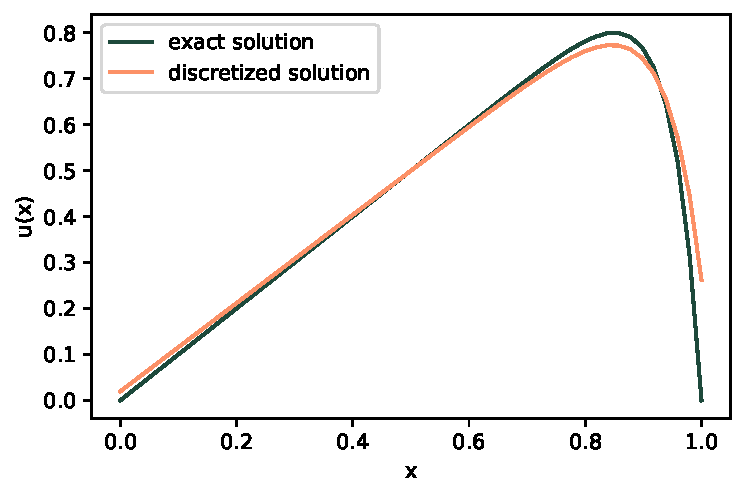
\includegraphics{4_convecDiff_files/figure-pdf/fig-th_vs_dis-output-1.pdf}

}

\subcaption{\label{fig-th\_vs\_dis-1}\(b = 0.05\), \(n=50\).}

\end{minipage}%
%
\begin{minipage}{0.50\linewidth}

\centering{

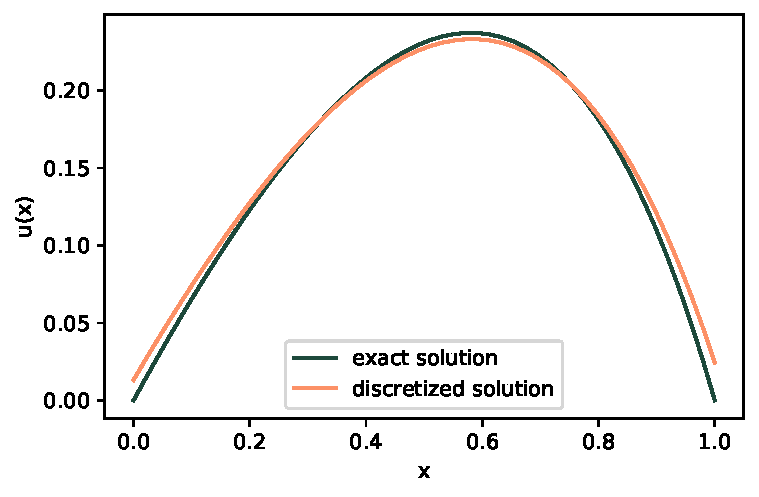
\includegraphics{4_convecDiff_files/figure-pdf/fig-th_vs_dis-output-2.pdf}

}

\subcaption{\label{fig-th\_vs\_dis-2}\(b = 0.5\), \(n=50\).}

\end{minipage}%

\caption{\label{fig-th_vs_dis}Exact and discretized solution of the
convection diffusion equation, for different parameters.}

\end{figure}%

To solve this linear system, we use the method highlighted before. To
make it easier for later, we choose to scale \(N\) so that its diagonal
elements are \(1\). This allows us to have all eigenvalues in the circle
centered around \(1\) with radius \(1\) independently of the
parametrization. Setting
\(\eta = \frac{1}{\Delta x} + \frac{2b}{\Delta x^2}\), solving
Equation~\ref{eq-UnscaledSystem} is equivalent to solving the system

\begin{equation}\phantomsection\label{eq-test_problem_scaled_system}{
\mathbfit{M} \mathbfit{u} = \mathbfit{e},
}\end{equation}

where with \(\mathbfit{M} = \frac{\mathbfit{N}}{\eta}\),
\(\mathbfit{e} = \frac{\mathbfit{d}}{\eta}\). The eigenvalues of
\(\mathbfit{N}\) are also scaled by \(\frac{1}{\eta}\), and therefore
\(-\mathbfit{M}\) is stable, assuming it is non singular. We are now
ready to solve the system iteratively using an ODE solver. To do that,
we introduce a (pseudo) time variable \(t\) and we consider the ODE

\begin{equation}\phantomsection\label{eq-test_problem_diff_eq}{
\mathbfit{u'(t)} = \mathbfit{e} - \mathbfit{Mu(t)}.
}\end{equation}

where \(\mathbfit{M}\) and \(\mathbfit{e}\) depends on both \(n\) and
\(b\). From now on, we call \(b\) and \(n\) the problem parameters. We
can use Theorem~\ref{thm-steadyState} with the non singularity
assumption to guarantee that \(\mathbfit{u(t)}\) converges to a steady
state independently of its chosen initial value. In the next chapter, we
introduce a numerical method to solve this differential equation, which
we will use in this thesis.

\begin{remark}
The convection diffusion equation is derived in {[}13{]} , chap.~3 from
the continuity equation for a scalar quantity \(u\) and is

\[
\frac{\partial u}{\partial t} + \Delta.(\vec{v}u - \nabla(Du)) = R.
\]

We will assume that the quantity \(u\), is the temperature in Kelvin,
and has the S.I unit \(K\). The physical quantities are:

\begin{itemize}
\tightlist
\item
  \(\vec{v}\), which is the velocity of the medium the quantity is in,
  in \(\text{ms}^{-1}\). (the advection/convection).
\item
  \(D\) is the diffusion coefficient, in \(\text{m}^2\text{s}^{-1}\).
\item
  \(R\) is governing whether the quantity is created when \(R>0\), or
  destructed when \(R<0\). The unit is \(K\text{s}^{-1}\).
\end{itemize}

We can now simplify the equation by considering it in a single dimension
\(x\)

\[
\frac{\partial u}{\partial t} + \frac{\partial}{\partial x}.(vu - \frac{\partial}{\partial x}(Du)) = R.
\]

This further simplifies to \(u_t + vu_x - Du_{xx} = R\).

Then, in the steady state, \(u_t = 0\) so we get

\[
u_x = \frac{D}{v}u_{xx} + \frac{R}{v},
\]

and we recognize Equation~\ref{eq-convec_diff_steady}, with
\(b = \frac{D}{v}\), and \(1 = \frac{R}{v}\). This also means that we
``lose'' two parameters in the studied test problem for simplification
purposes. Nevertheless, this can be used to give some degree of
intuition behind Figure~\ref{fig-th_vs_dis}. When the diffusion is high
compared to the convection, the quantity is more centered, but on the
other hand, when the convection speed is high compared to the diffusion,
the quantity \(u\) is ``flushed'' to the right (assuming \(v>0\)).
\end{remark}

\bookmarksetup{startatroot}

\chapter{Explicit Runge-Kutta Method}\label{explicit-runge-kutta-method}

\section{A small introduction to explicit Runge-Kutta
methods}\label{a-small-introduction-to-explicit-runge-kutta-methods}

This section aims to introduce explicit Runge-Kutta methods, {[}14, Ch.
3{]}, which we use in this paper. We consider solving a generic initial
value problem of the form

\[
y'(t) = f(t,y(t)), \quad y(0) = y_0.
\]

If we know, for an instant \(t_n\), the value for \(y(t_n)\), we can
compute the value of \(y\) at instant \(t_{n+1} = t_n +\Delta t\) by
integrating

\[
y(t_{n+1}) = y(t_n) + \int_{t_n}^{t_{n+1}}f(u,y(u))\; du,
\]

and with the change of variable \(u = t_n + \Delta t\tau\), we have

\[
y(t_{n+1}) = y(t_n) + \Delta t\int_0^1f(t_n+\Delta t\tau,y(t_n+\Delta t\tau)) \; d\tau.
\] The problem is finding a suitable way to compute the integral above.
An elementary approach is to use the current value of \(f(t_n,y(t_n))\)
and to treat \(f\) as constant, thus defining the sequence

\[
y_{n+1} = y_n + \Delta tf(t_n,y_n),
\]

where \(y_{n} \approx y(t_{n})\), \(y_0 = y(0)\). This is the explicit
Euler's method. We now want to exploit quadrature formulas for numerical
integration. Let \(c_j \in [0,1], j=1,2,\dots, \nu\), where \(\nu\) is
an integer, be the nodes in the quadrature formula, with their
associated weight \(b_j, j=1,2,\dots, \nu\). A quadrature formula for
the integral is then of the form

\[
\int_0^1 f(t_n+\Delta t \tau,y(t_n+\Delta t\tau))\; d\tau \approx \sum_{j=1}^\nu b_j f(t_n + \Delta t c_j,y(t_n+\Delta t c_j)).
\]

This is all well and good, except that we have to know the values
\(y(t_n+\Delta c_j)\), which we do not possess. We can however, play
pretend and compute an approximation of these values
\(\xi_j \approx y(t_n+\Delta t c_j), j=1,\dots, \nu\). The \(\xi_j\) are
called \emph{stage values}. {[}15{]}. The main idea to use the
\(\xi_i\)'s to compute \(\xi_j\), using a linear combination of the
terms \(f(t_n + \Delta t c_j, \xi_i)\). That is

\[
\xi_i = y_n + \Delta t \sum_{j=1}^\nu a_{ij}f(t_n+\Delta t c_j, \xi_j),
\]

for \(i = 1,\dots, \nu\), where the \(a_{ij}\) are some well chosen
values, which is not in scope of this thesis. To simplify notation, we
note \(A\) as the square array containing the \(a_{ij}\) parameters,
that is \(A_{ij} = a_{ij}\), \(c = (c_1,\dots,c_\nu)^\intercal\) the
vector of nodes, and \(b = (b_1,\dots, b_\nu)^\intercal\) the vector of
weights. An RK method is then written in the form of the following
array, also called a Butcher tableau:

\[
\renewcommand\arraystretch{1.2}
\begin{array}
{c|c}
c & A\\
\hline & b^\intercal
\end{array}.
\]

We remark that if, for any \(j\geq i\), \(a_{ij} \neq 0\), then we will
need to know \(\xi_j\) to compute \(\xi_i\), which involves solving an
equation, making the method \emph{implicit}. We consider here
\emph{explicit} methods, where we can compute \(\xi_{i+1}\) if we know
\(\xi_j, j = 1 , \dots , i-1\). Since we know \(f(t_n,y_n)\), we choose
\(a_{11} = 0\) and \(c_1 = 0\). An explicit RK method is then of the
form

\[
y_{n+1} = y_n + h\sum_{j=1}^\nu b_j f(t_n+\Delta t c_j,\xi_j),
\]

where the stage values \(\xi_j\) are computed sequentially as follow

\begin{align*}
\xi_1 &= y_n,\\
\xi_2 &= y_n + \Delta t a_{2,1}f(t_n,\xi_1),\\
\xi_3 &= y_n + \Delta t a_{3,1}f(t_n,\xi_1) +  \Delta t a_{3,2}f(t_n+\Delta t c_2,\xi_2),\\
\vdots\\
\xi_\nu &= y_n + \Delta t \sum_{j=1}^{\nu-1} a_{\nu,j}f(t_n + \Delta t c_j,\xi_j).
\end{align*}

\section{Application to the test
problem}\label{sec-RK_solver_test_problem}

We now have to solve the ODE \(u'(t) = e - Mu(t)\) where \(M\) depends
on the problem parameters \(b\) and \(\Delta x = 1 / (n+1)\), and \(n\)
is the chosen number of subdivisions of \([0,1]\). We consider in this
thesis the following RK method with two stages {[}15{]};

\[
\begin{array}
{c|cc}
0 & &\\
 \alpha & \alpha & \\
\hline & 0 & 1
\end{array}.
\]

\begin{remark}
This RK method can be extended to more stages. We only need the last
stage value to compute the time step update, and we only need to compute
the stage values sequentially using only the last stage value
calculated. This makes it possible, when programming the method, to
simply to do the update of the variable \(\xi\) in place inside the
computer memory. Such methods are thus memory efficient.
\end{remark}

This solver has two parameters, namely the (pseudo) time step
\(\Delta t\) and \(\alpha\), where \(\alpha \in [0,1]\).

The goal is for the solver to converge to a steady state solution in as
few iterations as possible.

\subsection{A note on stability}\label{a-note-on-stability}

Using the same notation as before for the stage values and the studied
RK method, for the equation \(u'(t) = f(t,u(t))\), we have
\(\xi_1 = u_n\),

\[
\xi_2 = u_n + \Delta t \alpha f(t_n,\xi_1) = u_n + \Delta t \alpha f(t_n,u_n).
\]

The update is thus;

\[
u_{n+1} = u_n + \Delta t f(t_n+\alpha \Delta t, \xi_2).
\]

In the test problem case,
\(f(t_n,\mathbfit{u}_n) = \mathbfit{e} - \mathbfit{Mu}_n\), and we get
the update

\[
\mathbfit{u}_{n+1} = \mathbfit{u}_n + \Delta t\left[\mathbfit{e}-\mathbfit{M}(\mathbfit{u}_n+\alpha\Delta t(\mathbfit{e}-\mathbfit{Mu_n}))\right].
\]

After a few lines of computation, we get the following iteration,

\begin{equation}\phantomsection\label{eq-stationary_linear_iter}{
\mathbfit{u}_{n+1} = \left[\mathbfit{I}- \Delta t(\mathbfit{I}- \alpha \Delta t \mathbfit{M})\mathbfit{M}\right]\mathbfit{u}_n + \left[\Delta t(\mathbfit{I} - \alpha \Delta t \mathbfit{M})\right]\mathbfit{e}.
}\end{equation}

This iteration is of the form
\(\mathbfit{u}_{n+1} =\mathbfit{Ku}_n  + \mathbfit{Le}\), where

\begin{equation}\phantomsection\label{eq-L}{
\mathbfit{L} = \Delta t\left[ \mathbfit{I} - \alpha \Delta t \mathbfit{M}\right]
}\end{equation} and \begin{equation}\phantomsection\label{eq-K}{
\mathbfit{K} = \mathbfit{I}- \mathbfit{LM} = \left[\mathbfit{I}- \Delta t(\mathbfit{I}- \alpha \Delta t \mathbfit{M})\mathbfit{M}\right].
}\end{equation}

We recognize this iteration as a linear stationary iteration, which
converges to a unique fixed point for any starting value
\(\mathbfit{u}_0\) if and only if \(\rho(K)<1\), {[}16, Ch. 2.2{]},
where \(\rho(\mathbfit{K})\) is the spectral radius of \(\mathbfit{K}\).
Furthermore, this iteration satisfies the consistency requirement
\(\mathbfit{K} = \mathbfit{I}-\mathbfit{LM}\), so the fixed point, when
it exists, is \(\mathbfit{u}^* = \mathbfit{M}^{-1}\mathbfit{e}\).

\begin{remark}
One may remark that \(\mathbfit{K} = p(\Delta t \mathbfit{M})\) with
\(p(z) = 1- z + \alpha z^2\) a polynomial. This polynomial is also the
stability polynomial of the RK method {[}15{]}.
\end{remark}

\subsection{Residual ratios}\label{residual-ratios}

We have shown in the last section the sufficient and necessary condition
for the solver to converge to the desired solution
\(\mathbfit{u}^* = \mathbfit{M}^{-1}\mathbfit{e}\). This condition is
that \(\rho(\mathbfit{K})<1\). The spectral radius can be computed with
power iterations {[}17, Pt. V{]}, but this is an expensive task that we
may not be able to do in practice. Furthermore, the derivation of
\(\mathbfit{K}\) is specific to this method, and may not be as
accessible with other methods. We instead turn our attention to another
method.

We set \(\mathbfit{u}_0 = \mathbfit{e}\) as an initial value. We define
the relative residual after \(k\) steps as

\begin{equation}\phantomsection\label{eq-relative_residual}{
r_k = \frac{||\mathbfit{M}\mathbfit{u}_k - \mathbfit{e}||}{||\mathbfit{e}||},
}\end{equation}

where \(||.||\) is the 2-norm.

If the solver we chose is stable, then \(||r_k|| \to 0\) as
\(k \to \infty\). We define now the residual ratio at step \(k\) to be
the ratio of the residuals at step \(k\) and \(k-1\). That is

\begin{equation}\phantomsection\label{eq-residual_ratio_equation}{
\rho_k = \frac{r_k}{r_{k-1}} = \frac{||\mathbfit{Mu}_k - \mathbfit{e}||}{||\mathbfit{Mu}_{k-1}-\mathbfit{e}||}.
}\end{equation}

Note that the residual ratio depends on both the problem parameters and
the solver parameters. It will be useful in future sections to make that
relation evident by using the notation
\(\rho_{k,b,n}(\alpha, \Delta t)\).
Figure~\ref{fig-residual_ratio_evolution} shows the evolution of the
relative residual, as well as the residual ratio for specific
parameters. After a certain number of iterations, the residual ratio
stabilizes. This can be however be after a large amount of iterations,
so the rate of convergence can be costly to compute.

\begin{figure}

\centering{

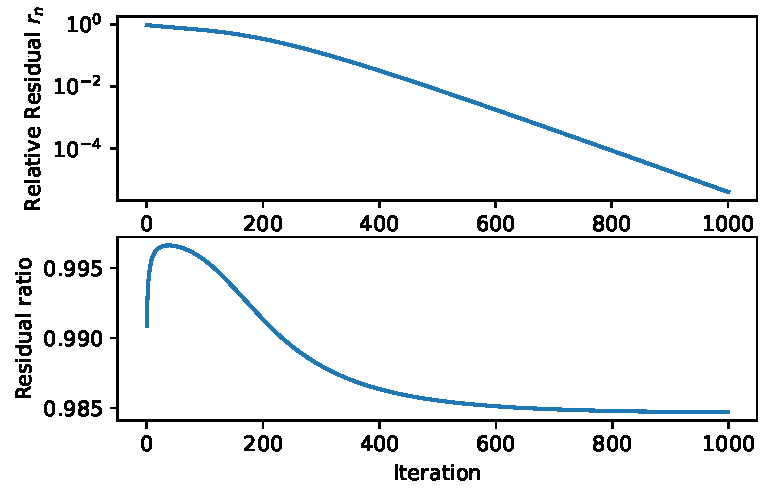
\includegraphics{5_solverExploration_files/figure-pdf/fig-residual_ratio_evolution-output-1.pdf}

}

\caption{\label{fig-residual\_ratio\_evolution}Evolution of the residual
norm over iteration, with problem parameters \(n = 50\) and
\(b = 0.05\), and RK parameters \(\Delta t = 1\) and \(\alpha = 0.2\).}

\end{figure}%

\section{A small experiment}\label{sec-small_experiment}

We are interested in finding the best parameters \((\Delta t, \alpha)\)
to use for some specific problem parameters \((b,n)\). Ideally, we
should minimize the asymptotic residual ratio \(\rho_\infty\), but this
is computationally intensive, so we restrict ourselves to minimizing the
residual ratio \(\rho_k\) after a fixed amount of iterations.

As we've seen in Figure~\ref{fig-residual_ratio_evolution}, \(\rho_k\)
can vary quite a bit depending on \(k\), so we decide to investigate the
residual ratio after 10 iterations and 100 iterations. We set the
problem parameters \(b = 0.05\), and \(n = 100\), and we plot
\(\rho_{k,0.05,100}(\Delta t, \alpha)\) for different values of \(k\).
This is achieved by making a linear grid for parameters \(\Delta t\) and
\(\alpha\) of size \(100\times 100\), where \(\alpha\) varies between
\(0\) and \(1\), and \(\Delta t\) varies between \(0\) and \(5\), then
computing the residual ratios on that grid.

We wish to find the optimal parameters for this specific problem, that
is, the ones that minimize \(\rho_{k}\), for different values of \(k\).
We are also interested in seeing how much the optimal parameters depend
on \(k\).

After 100 iterations, we see that we need to choose the parameters in
more narrow region than after 10 iterations to get \(\rho_{100}<1\),
suggesting that convergence of the solver may not hold even if it seems
to hold for the first few iterations. However, this doesn't seem to be
the case when we consider higher values of \(k\). Nevertheless, we can
see how the solver parameters interact with the residual ratio.

By doing this experiment, we motivate the following method: using a grid
search, look for the solver parameters that minimize \(\rho_k\), where
\(k\) has to be chosen as low as possible to minimize computing time,
but also high enough to ensure that the solver won't diverge after more
iterations. This method however need to be repeated for each individual
problem parameters. We therefore explore a possible solution to this
problem by using a reinforcement learning algorithm to ``learn'' the
optimal solver parameters \(\alpha\) and \(\Delta t\), as a function of
the problem parameters \(b\) and \(n\).

\begin{figure}

\begin{minipage}{0.50\linewidth}

\centering{

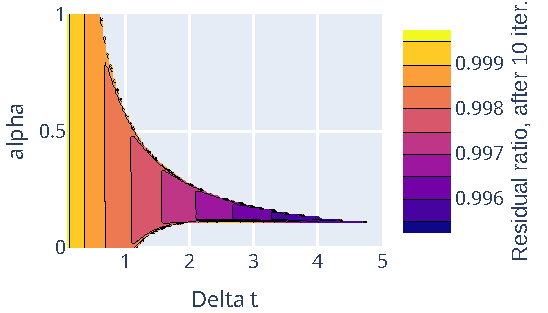
\includegraphics{images/res_ratio10.pdf}

}

\subcaption{\label{fig-res\_ratio10}\(\rho_{10}\)}

\end{minipage}%
%
\begin{minipage}{0.50\linewidth}

\centering{

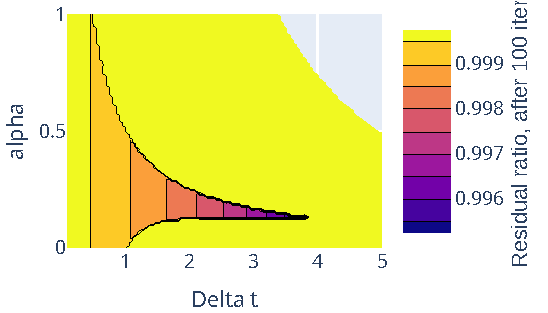
\includegraphics{images/res_ratio100.pdf}

}

\subcaption{\label{fig-res\_ratio100}\(\rho_{100}\)}

\end{minipage}%
\newline
\begin{minipage}{0.50\linewidth}

\centering{

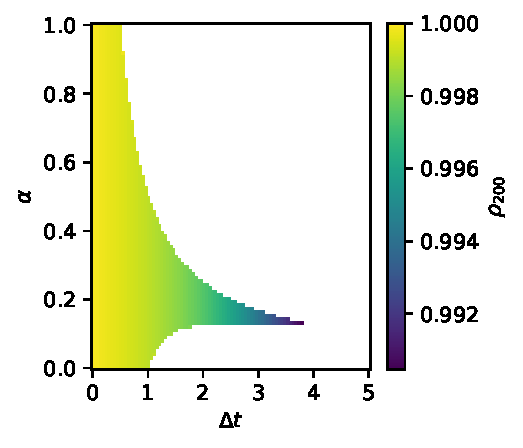
\includegraphics{images/res_ratio200.pdf}

}

\subcaption{\label{fig-res\_ratio200}\(\rho_{200}\)}

\end{minipage}%
%
\begin{minipage}{0.50\linewidth}

\centering{

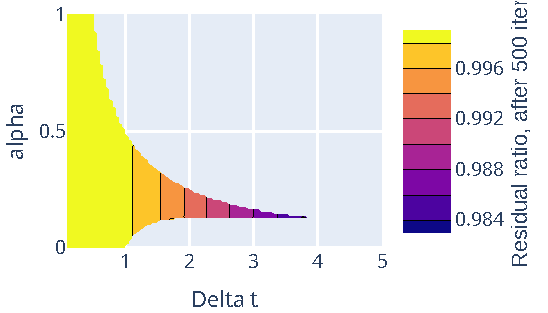
\includegraphics{images/res_ratio500.pdf}

}

\subcaption{\label{fig-res\_ratio500}\(\rho_{500}\)}

\end{minipage}%

\caption{\label{fig-res_ratio_comparison}Contour plot of some residual
ratios \(\rho_k\), for different \(k\) after different number of
iterations, for the specific problem parameters \(n = 100\) and
\(b=0.05\). Note that the area in white is where \(\rho_k > 1\).}

\end{figure}%

\bookmarksetup{startatroot}

\chapter{Basics of Reinforcement Learning
(RL)}\label{basics-of-reinforcement-learning-rl}

In this section, we outline the main ideas behind reinforcement learning
and how they can be applied in the context of this thesis. The reader
familiar with the material may skip this section.

\section{A non mathematical, yet delicious
example!}\label{a-non-mathematical-yet-delicious-example}

In Reinforcement Learning tasks, we are training an \emph{agent} that
interacts with its \emph{environment} by taking decisions. In this
example, we are the agent, and the environment is the kitchen. Suppose
we want to cook a delicious meal. At any point in time, we are making
decisions such as;

\begin{itemize}
\tightlist
\item
  Which ingredients we use. Do we use tofu or seitan? Do we add spice or
  more chili pepper? When do we incorporate the sauce?
\item
  Which cookware we use? Cast iron, or non-stick pan?
\item
  Whether to put the oven to \(200^\circ C\) or \(220^\circ C\).
\item
  Or simply do nothing!
\end{itemize}

All of these decisions, which we will call \emph{actions} from now on,
are taken based on the current \emph{state} of the environment, that is
the cooking process. How we decide which \emph{action} to take given a
current \emph{state} will be called the \emph{policy} from now on.

After each action, the cooking process gets to a new \emph{state} and we
taste the meal. By tasting it, we get a \emph{reward} that depend on how
well we did. Maybe the food started to burn in which case we get a
negative reward, or maybe we made the food tastier, in which case we get
a positive reward. In this example, there is a \emph{starting state},
where we decide to cook something, and a \emph{terminal state}, in which
we finished cooking and get to enjoy the meal.

But how do we learn how to cook, how do we know what \emph{action} to
take at a specific \emph{state}? That is, how do we learn the
\emph{policy}? We learn it by getting feedback, which is defined by the
\emph{reward} we get after each action. Some of those rewards are
immediate, for example, if we add some spices to our food and it tastes
better. We want to have a \emph{policy} that maximizes the total
\emph{rewards} we get over a entire cooking session. This also mean that
we have to balance how we prefer the immediate rewards against the
future rewards. For example, adding a spice may make the meal taste
better in the short term, for which we get a reward, but it may clash
later when we add other ingredients, leading to a worse meal and worse
\emph{rewards} down the line.

Each time we cook, we learn what works and what doesn't, and remember
that for any future time we cook. But, if we want to get better at
cooking, we must not just repeat the \emph{actions} that worked! We also
have to take some risks, and \emph{explore} the potential actions we can
take at each state! On the other hand, we still need to rely and
\emph{exploit} what we know. There is a balance to find between
\emph{exploitation} and \emph{exploration} so as to learn as fast as
possible.

\section{Another example: Leonardo the
rabbit}\label{another-example-leonardo-the-rabbit}

The last example is an intuitive way of thinking of reinforcement
learning as similar to the way we animals learn about the world and its
processes. The ideas behind reinforcement learning borrow a lot from the
fields of psychology and neuroscience{[}18{]}, and modelling how we
learn is a gargantuan task that is, for this very reason, outside of the
scope of this thesis!

We turn our attention to a more modest example that is much easier to
model, and is an example that one can find in a lot of reinforcement
learning books{[}8{]}, {[}19{]}. We consider the case of Leonardo the
rabbit. Leonardo, the agent, is situated in the outside world, which is
represented as a \(3\times 3\) grid (the environment). He wants to get
to the carrot at the bottom right as fast as possible. To help Leonardo
get to his meal, we will use reinforcement learning.

\subsection{States}\label{states}

The first thing we do is give a number to each box in the grid, from
\(1\) to \(9\). We call the set of all boxes number as the state set,
which we denote by \(\mathcal{S}\). In this example,
\(\mathcal{S} = \{1,2,\dots,9\}\) (see Figure~\ref{fig-gridworld1}). A
state is defined as any element in the state set, which we denote by
\(s\in\mathcal{S}\). The state is the box Leonardo is in.

\begin{figure}

\centering{

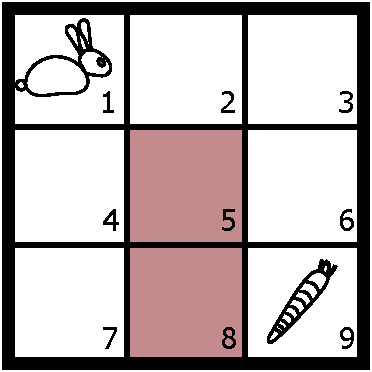
\includegraphics{images/gridworld.pdf}

}

\caption{\label{fig-gridworld1}Can you help special agent Leonardo get
to his carrot? The grid environment, where our fluffy friend is situated
in. His state is \(s=1\).}

\end{figure}%

\subsection{Actions}\label{actions}

Leonardo, in this grid, can move in any 4 directions, that is left,
right, up or down. We call this the action set \(\mathcal{A}\), and in
this example \(\mathcal{A} = \{\text{left,right,up,down}\}\). An action
is defined as any element in the action set, which we denote by
\(a\in\mathcal{A}\).

\subsection{State transitions}\label{state-transitions}

At this point, we can introduce a time variable \(t\). The initial time
is set to \(t=0\), and, after Leonardo takes an action \(t\) moves
forward by \(1\), and he finds himself in a new state. This is what we
call a state transition(see Figure~\ref{fig-gridworld_transition}).

We want to keep track of Leonardo positions and actions over time, which
is why we denote the state Leonardo is in at time \(t\) by \(S_t\), and
the action he takes by \(A_t\). In this example, there is the initial
state \(S_0 = 1\).

\begin{remark}
\(S_t\) and \(A_t\) are random variables, which is we note in uppercase.
Specific observations of \(S_t\) and \(A_t\) will be in lowercase, that
is respectively \(s_t\) and \(a_t\).
\end{remark}

\begin{figure}

\centering{

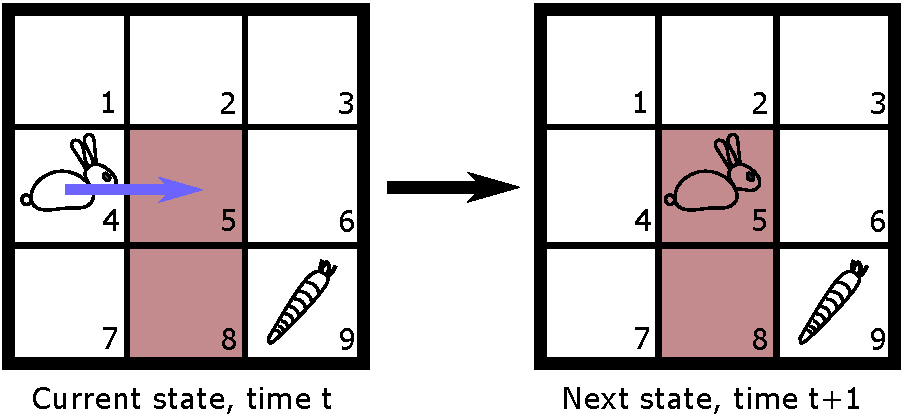
\includegraphics{images/gridworld_transition.pdf}

}

\caption{\label{fig-gridworld\_transition}An example of state
transition. Leonardo, being at the state \(s_t = 4\), takes the action
\(a_t = \text{right}\). After this action, he is at the state
\(s_{t+1} = 5\). Leonardo gets the reward \(r_{t+1} = -5\).}

\end{figure}%

\subsection{Policy}\label{policy}

Leonardo, as the agent, only has access to his current state \(S_t\). He
has to take an action \(A_t\), but how does he know which action to
take? To do that, he uses a policy, which we denote by a function
\(\pi\). More formally, \(\pi\) is a function that defines the
probability of taking the action \(A_t = a\) if the state is
\(S_t = s\). We denote this by \(\pi(a|s)\).

Suppose for example that \(S_t = 3\). Leonardo has no idea of where the
carrot is, but he knows that he can not go up nor to the right, so his
policy is to go down, or right at random. Then:

\begin{itemize}
\tightlist
\item
  The probability to go right is \(\pi(\text{right}, 3) = 0.5\).
\item
  The probability to go down is \(\pi(\text{down}, 3) = 0.5\).
\end{itemize}

More specifically, for any state \(s\), we define the conditional
probability mass function \(\pi(a|s) = \Pr(A_t = a | S_t = s)\), where
\(\Pr\) denote a probability. Hence, for any fixed state \(s\),
\(\sum_{a\in\mathcal{A}} \pi(a|s) = 1\).

\begin{remark}
We will assume that Leonardo only cares about what his current state is
to take an action, and not for how long he has been in the grid. This
makes the policy independent of the time \(t\).
\end{remark}

\subsection{Rewards}\label{rewards}

While Leonardo only takes actions by looking at his current state, he
still wants to get to the carrot as fast as possible. He knows his
current state \(s_t\) and takes the action \(a_t\). Doing so, he ends up
in the state \(s_{t+1}\) and he gets a reward.

\begin{itemize}
\tightlist
\item
  The red colored box are difficult to get in, so if he ends up on one
  of the red colored box, he gets a reward of \(-5\). This is for
  example the case in Figure~\ref{fig-gridworld_transition}.
\item
  If he ends up on the carrot, he gets a reward of \(+5\).
\item
  If he ends up in any other state, he gets a reward of \(-1\), as he
  does not want to lose time.
\end{itemize}

More formally, we denote the reward Leonardo gets after taking the
action \(A_t\) from the state \(S_t\) by \(R_{t+1}\). The set of all
possible rewards is denoted by \(\mathcal{R}\). Here
\(\mathcal{R} = \{-1,5,-5\}\). \(R_t\) is again a random variable and we
denote an observation of the reward at time \(t\) by \(r_t\).

\subsection{State transitions and rewards
probabilities}\label{state-transitions-and-rewards-probabilities}

Suppose now that there is a teleporter in the 4th box. This teleporter
is however unreliable. Half the time, it teleports whoever steps in the
box to the \(9^{th}\) box, meaning Leonardo could potentially get
directly to his prize! The other half of the time, however, it teleports
the user to the \(7^{th}\) box.

Suppose now that Leonardo is at state \(s_t=1\), he takes the action
\(a_t = \text{down}\) to the teleporter(see
Figure~\ref{fig-gridworld_teleporter}). Then:

\begin{itemize}
\tightlist
\item
  The next state is \(s_{t+1} = 9\) with probability \(0.5\).
\item
  The next state is \(s_{t+1} = 7\) with probability \(0.5\).
\end{itemize}

But now, the reward he gets is random too!

\begin{itemize}
\tightlist
\item
  If he end up in the \(9^{th}\) box, \(r_{t+1} = 5\).
\item
  If the teleporter does not work and he ends up in the \(7^{th}\) box,
  \(r_{t+1} = -1\).
\end{itemize}

More specifically, this means that state transitions and rewards need to
be modelled by a probability, more specifically, the probability of
getting a reward \(r\in\mathcal{R}\), and that the next state is
\(s'\in\mathcal{S}\) given that the agent takes the action
\(a\in\mathcal{A}\) at the state \(s\in\mathcal{S}\). We formalize a
state transition probability as the conditional probability defined in
the sample space \(\mathcal{S}\times \mathcal{R}\)

\[
p(s',r|s,a) = \Pr(S_{t+1} = s', R_{t+1} = r | S_t = s, A_t = a).
\]

\begin{figure}

\centering{

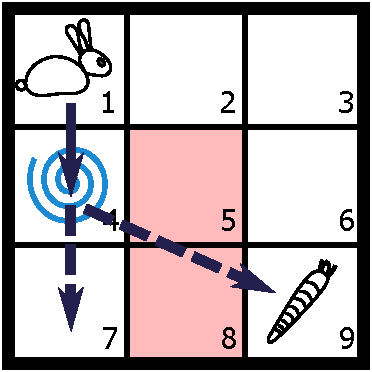
\includegraphics{images/bunny_teleporter.pdf}

}

\caption{\label{fig-gridworld\_teleporter}Will it be worth the risk?
Leonardo has taken the action \(a = \text{down}\) at the state \(s=1\).
There is a \(50\%\) chance he ends up right on his prize! The state
transition and reward probability is \(p(s'=9,r=5|s=1,a=down) = 0.5\).
Similarly, \(p(s'=7,r=-1|s=1,a=down) = 0.5\).}

\end{figure}%

\section{Finite Markov decision
process}\label{finite-markov-decision-process}

We formalize the above example by defining a Markov decision process
(MDP). This definition and the ones up until the end of this chapter are
adapted from {[}19{]}.

\begin{definition}[]\protect\hypertarget{def-Markov_decision_process}{}\label{def-Markov_decision_process}

\textbf{(Markov decision process)}. A finite Markov decision process
(MDP) is defined as a discrete time process, where we have:

\begin{itemize}
\tightlist
\item
  A finite set of all states \(\mathcal{S}\).
\item
  A finite set of all possible actions \(\mathcal{A}\).
\item
  A reward set \(\mathcal{R}(s,a)\), which contains the potential
  rewards received after taking any action \(a\in\mathcal{A}\) from any
  state \(s\in\mathcal{S}\).
\end{itemize}

We use the notation \(S_t, A_t\) as the state and action of the process
at time \(t\). The reward \(R_t\) is the reward received at time t.
\(S_t,A_t\) and \(R_t\) are random variables.

A Markov decision process also has a model, which consists of the state
and reward transition probabilities:

\begin{itemize}
\tightlist
\item
  The probability, given that the current state is \(s\), and that the
  action taken is \(a\), that the next state is \(s'\) and the next
  reward is \(r\). That is
  \(p(s',r|s,a) = \Pr(S_{t+1} = s', R_{t+1} = r | S_t = s, A_t = a)\).
\end{itemize}

Furthermore, a Markov decision process has a policy that governs, for
any state \(s\in\mathcal{S}\), the probability of taking action
\(a\in\mathcal{A}\), that probability is
\(\pi(a|s) = \Pr(A_t = a|S_t = s)\). We assume that the policy is not
dependent on time.

Finally, a Markov decision process has the Markov property, or lack of
memory. The state transition and rewards probabilities are only
dependent on the current state \(S_t\) and action \(A_t\), and not the
states and actions that preceeded. Mathematically,
\(\Pr(S_{t+1} = s', R_{t+1} = r|S_t, A_t, S_{t-1}, A_{t-1}, \dots , S_0, A_0) = \Pr(S_{t+1} = s', R_{t+1} = r | S_t, A_t)\).

\end{definition}

An example of Markov decision process with two states can be seen in
Figure~\ref{fig-MDP_example}.

\begin{figure}

\centering{

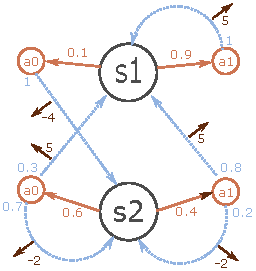
\includegraphics[width=0.4\textwidth,height=\textheight]{images/MDP.pdf}

}

\caption{\label{fig-MDP\_example}An example of a Markov decision process
with two states \(s_1\) and \(s_2\) and two possible actions \(a_0\) and
\(a_1\) for each states. The dashed lines represent the model
transitions. After each action, the process get to a new state and a
reward is given, here in dark red.}

\end{figure}%

\begin{remark}
The state space \(\mathcal{S}\) and the action space \(\mathcal{A}\) can
be finite or not. We only consider the case of finite Markov decision
process to make matters easier.
\end{remark}

\begin{remark}
The model in a Markov decision process is often impossible to define in
advance. This problem is remedied by using \emph{model free} algorithms.
\end{remark}

\section{State Value and Bellman
Equation}\label{state-value-and-bellman-equation}

We have a Markov decision process, which serves as a nice mathematical
formalization of an agent and its environment {[}8{]}. Now we want to
train the agent to make the best possible decisions? Answering this
question is the goal of the next sections.

We first define a trajectory. We denote by \(S_t\) the state of an agent
at instant \(t\). Then, according to the policy, this agent takes the
action \(A_t\). After taking this action, the agent is now at the state
\(S_{t+1}\), and it gets the rewards \(R_{t+1}\). Then the agent takes
action \(A_{t+1}\), and gets to a new state \(S_{t+2}\) with reward
\(R_{t+2}\). This continues indefinitely. We define the trajectory of an
agent with starting state \(S_t = s_t\) as the chain of states, actions
and rewards from time \(t\) onward:

\[
S_t = s_t,A_t \to R_{t+1},S_{t+1},A_{t+1} \to R_{t+2},S_{t+2},A_{t+2} \to \cdots,
\]

Note that, due to the Markov property and the fact that we assume the
policy is time independent, the starting value of \(t\) is not
important.

\begin{remark}
In some environments, it is natural for the agent to have a task that
has a starting state and a finishing states (for example, beginning a
cooking session and finishing it, or starting a game and winning/losing
at it.) We call these tasks \emph{episodic tasks} and in these cases, a
finite trajectory \(S_0,A_0 \to \dots \to S_T\) is also called an
\emph{episode}. In the cases where the task is such that no such state
can be defined, a trajectory is not finite and we call these tasks
\emph{continuing tasks}, which will be the case in this thesis.
\end{remark}

In reinforcement learning setting, we assume that we have no control of
the environment model (for example, one can not change the rules of a
game), but that we have control over the agent decisions (i.e the
policy) and how we reward that agent. The goal of any reinforcement
learning algorithm is thus to define the rewards properly and then to
find a policy that maximizes the rewards the agent gets. We now define
the discounted return along a trajectory,

\begin{definition}[]\protect\hypertarget{def-discount}{}\label{def-discount}

Let \(t = 0, 1, \dots\). The (discounted) return along the trajectory
\(S_t,A_t \to S_{t+1},A_{t+1}, R_{t+1} \to S_{t+2},A_{t+2}, R_{t+2} \to \dots\)
is the random variable given by

\[
G_t = R_{t+1} + \gamma R_{t+2} + \gamma^2 R_{t+3} + \dots = \sum_{k=0}^{+\infty}\gamma^k R_{t+1+k},
\]

where \(\gamma \in [0,1)\) is called the discount rate.

\end{definition}

\begin{remark}
By setting a discount rate that is less than 1 in continuing tasks, we
make sure that the discounted return is well defined in the case of
bounded rewards. Indeed, if, for any \(t\), \(|R_t|\leq M\), then
\(\sum_{k=0}^{+\infty}|\gamma^k R_{t+1+k}| \leq  \sum_{k=0}^{+\infty}\gamma^k M = \frac{M}{1-\gamma}\),
so the series is absolutely convergent.
\end{remark}

The \emph{discounted return} is thus the sum of rewards along a
trajectory, with a penalty for rewards far in the future, controlled by
the \emph{discount rate}. The discount rate is chosen depending on
whether we want the agent to favor short term rewards, in which case a
discount rate closer to \(0\) can be chosen, or long term rewards, with
a discount rate closer to \(1\).

Since the discounted return is a random variable, we can look at its
expectation, in particular, we are interested in its conditional
expectation, given a starting state \(S_t = s\). This expectation is
called the state value {[}8{]}.

\begin{definition}[]\protect\hypertarget{def-state_value}{}\label{def-state_value}

\textbf{State value} The state value of a state \(s\) is the function,
defined for any \(s\in\mathcal{S}\) as the conditional expectation of
the discounted return, given \(S_t = s\),

\[
v_\pi(s) = E[G_t|S_t = s] = E[R_{t+1} + \gamma R_{t+2} + \gamma^2 R_{t+3} + \dots | S_t = s],
\]

where \(\pi\) is a given policy.

\end{definition}

\begin{remark}
Once again, the Markov property and the time independence of the policy
mean that the state value does not depend on time.
\end{remark}

We remark that

\begin{align}   
G_t &= R_{t+1} + \gamma R_{t+2} + \gamma^2 R_{t+3} + \dots \nonumber\\
&=R_{t+1} + \gamma \left(R_{t+2} + \gamma R_{t+3}+ \dots \right) \nonumber\\
&=R_{t+1} + \gamma G_{t+1}.
\end{align}

This expression of the return can be used in conjunction with the
definition of the state value above to get

\begin{equation}\phantomsection\label{eq-state_value_part1}{
v_\pi(s) = E[G_t|S_t = s]= E[R_{t+1}| S_t = s] + \gamma E[G_{t+1} | S_t = s].
}\end{equation}

The first term is the expectation of immediate reward, following a
certain policy \(\pi\), the second is the expectation of future rewards.
Let us expand on that formula a bit more. We now make use of the ``law
of total expectation'':

\begin{theorem}[]\protect\hypertarget{thm-total_expectation}{}\label{thm-total_expectation}

Let \(X\) and \(Y\) be random variables, and suppose \(E[|Y|]<\infty\).
Then \[
E[Y] = E\left[E[Y|X]\right]
\]

\end{theorem}

Using this, the expectation of immediate reward is

\[
E[R_{t+1}| S_t = s] = E\big[E[R_{t+1}|S_t = s,A_t]\big] = \sum_{a\in\mathcal{A}}\pi(a|s)\sum_{r\in\mathcal{R}} \sum_{s'\in \mathcal{S}}rp(s',r|s,a).
\]

We now develop the second part in the RHS of
Equation~\ref{eq-state_value_part1}, and use the law of total
expectation again to get

\[
E[G_{t+1} | S_t = s] = E\big[E[G_{t+1} | S_t = s , S_{t+1}]\big] = \sum_{s'\in\mathcal{S}}p(s'|s)E[G_{t+1}|S_t = s, S_{t+1} = s'],
\]

where
\(p(s'|s) = \sum_{a\in\mathcal{A}} \sum_{r\in\mathcal{R}}p(s',r|s,a)\pi(a|s)\)
is the probability of the next state being \(s'\) if the current state
is \(s\). Because of the Markov property of the MDP, we can remove the
conditioning \(S_t = s\) and thus,
\(E[G_{t+1}|S_t = s, S_{t+1} = s'] = E[G_{t+1}|S_{t+1} = s] = v_\pi(s')\).
Then \begin{equation}\phantomsection\label{eq-state_value_part2}{
E[G_{t+1} | S_t = s] = \sum_{s'\in\mathcal{S}}\sum_{a\in\mathcal{A}}\sum_{r\in\mathcal{R}}v_\pi(s')\pi(a|s)p(s',r|s,a).
}\end{equation}

Putting Equation~\ref{eq-state_value_part1} and
Equation~\ref{eq-state_value_part2} together, we get Bellman's equation:

\begin{equation}\phantomsection\label{eq-Bellman}{
v_\pi(s) = \sum_{a\in\mathcal{A}}\sum_{r\in\mathcal{R}}\sum_{s'\in\mathcal{S}}\pi(a|s)p(s',r|s,a)\left[ r + \gamma v_\pi(s')\right].
}\end{equation}

\begin{remark}
The Bellman equation depends on the given policy and gives a recursive
relation for the state values. Solving this equation is called policy
evaluation which involves fixed point iterations (see example below).
\end{remark}

\begin{example}[]\protect\hypertarget{exm-the_example}{}\label{exm-the_example}

We can directly derive the state values in the MDP in
Figure~\ref{fig-MDP_example}. We remark that in this example, given a
specific state transition, the reward we get is deterministic, which
simplifies the computations.

In particular, for the state \(s_2\), There are two possible actions
\(a_0\) and \(a_1\) we can take. The policy is to take action \(a_0\)
with a probability \(0.6\), and action \(a_1\) with a probability
\(0.4\). When we take for example action \(a_0\), the probability of the
next state being \(s_1\) is \(0.3\), in which case the reward is \(5\).
Proceeding similarly for all the possible actions and rewards, we get

\begin{align*}
v_\pi(s_2) &= \sum_{a=0}^1\sum_{r\in\mathcal{R}}\sum_{s'=1}^2\pi(a|s)p(s',r|s_2,a)\left[ r + \gamma v_\pi(s')\right]\\
&= 0.6 \sum_{r\in\mathcal{R}}\sum_{s'=1}^2 p(s',r|s_2,a=0)\left[ r + \gamma v_\pi(s')\right] + 0.4 \sum_{r\in\mathcal{R}}\sum_{s'=1}^2 p(s',r|s_2,a=1)\left[ r + \gamma v_\pi(s')\right]\\
&= 0.6 \left[0.3(5 + \gamma v_\pi(s_1)) + 0.7(-2 + \gamma v_\pi(s_2))\right] + 0.4\left[ 0.2(-2 + \gamma v_\pi(s_2)) + 0.8(5+\gamma v_\pi(s_1) \right].
\end{align*}

After some computations, we end up with

\[
v_\pi(s_2) = 1.5 + \gamma (0.5,0.5)\begin{pmatrix}
v_\pi(s_1) \\
v_\pi(s_2)
\end{pmatrix}.
\]

Similarly
\(v_\pi(s_1) = 4.1 + \gamma(0.9,0.1)(v_\pi(s_1),v_\pi(s_2))^\intercal\).
This leads to the system:

\[
\begin{pmatrix}
v_\pi(s_1)\\
v_\pi(s_2)
\end{pmatrix} = \begin{pmatrix}
4.1\\
1.5
\end{pmatrix} + \gamma \begin{pmatrix}
0.9 & 0.1\\
0.5 & 0.5
\end{pmatrix}\begin{pmatrix}
v_\pi(s_1)\\
v_\pi(s_2)
\end{pmatrix}.
\]

We stop here to remark that this equation is of the form
\(v_\pi = r_\pi + \gamma \mathbfit{P}_\pi v_\pi\). \(\mathbfit{P}_\pi\)
can be related to a state transition matrix in a markov chain and is row
stochastic. Furthermore, since \(\gamma<1\), we motivate solving the
equation by using fixed point iterations. This is the main idea behind
\emph{dynamic programming} {[}20{]}. In this case, we can simply solve
the system directly. For example, with \(\gamma=0.5\), we get the state
values \(v_\pi(s_1) = 7.875\), \(v_\pi(s_2) = 4.625\).

\end{example}

\section{Action Value}\label{action-value}

The state value gives information about a specific state, however, we
are also often interested in knowing how much we stand to gain by taking
a particular action at a particular state. This lead to the definition
of the action value.

\begin{definition}[]\protect\hypertarget{def-action_value}{}\label{def-action_value}

\textbf{Action value} The action value is defined as the expectation of
discounted return \(G_t\), given a specific action \(a\), taken at the
current state \(s\):

\[
q_\pi(a|s) = E\left[G_t|A_t=a,S_t=s\right] = E\left[\sum_|A_t=a,S_t=s\right],
\]

where \(G_t = R_{t+1} + \gamma R_{t+2} + \gamma^2R_{t+3} + \dots\).

\end{definition}

We also have, from Definition~\ref{def-state_value}, and the law of
total expectation,

\[
v_\pi(s) = E[G_t|S_t = s] = E\left[E[G_t|S_t = s, A_t = a]\right].
\]

Then, \[
v_\pi(s) = \sum_{a\in\mathcal{A}}\pi(a|s)E\left[G_t|S_t=s,A_t =a\right],
\]

and we can get the relation between state value and action value:

\begin{equation}\phantomsection\label{eq-state_value_action_relation}{
v_\pi(s) = \sum_{a\in\mathcal{A}} \pi(a|s)q_\pi(a|s).
}\end{equation}

We remark that by viewing \(\pi(a|s)\) as a probability mass function,
we can express the state values as another expectation:

\[
v_\pi(s) = E[q_\pi(a|s)],
\]

where \(A\) is random variable with p.m.f \(\pi(a|s)\). Actions values
are important in the sense that they tell us of the ``value of taking an
action over another'', and they appear naturally in almost all
reinforcement learning algorithms. One important thing to note is that,
by ``comparing'' Equation~\ref{eq-state_value_action_relation} and
Equation~\ref{eq-Bellman}, we get an equivalent definitions of the
action values as

\begin{equation}\phantomsection\label{eq-action_value_to_state_value}{
q_\pi(a|s) = \sum_{r\in\mathcal{R}}\sum_{s'\in\mathcal{S}}p(s',r|s,a)\left[ r + \gamma v_\pi(s')\right].
}\end{equation}

Equation~\ref{eq-action_value_to_state_value} means that if we have
access to the state values, we can compute the action values, while
Equation~\ref{eq-state_value_action_relation} works in the opposite way,
deriving state values from the action values.

\begin{remark}
A more rigorous approach to derive
Equation~\ref{eq-action_value_to_state_value} would be similar to how we
derive Bellman's equation.
\end{remark}

\section{Optimal policy and value
iteration}\label{optimal-policy-and-value-iteration}

Now that we have defined the state values, we want to find a policy that
maximizes them, that is, find a policy which we denote by \(\pi^*(a,s)\)
such that, for any state \(s\) and for any policy \(\pi(a|s)\),
\(v_{\pi^*}(s)\geq v_\pi(s)\). It turns out that not only this optimal
policy exist, but that we can find it by repeating the following steps,
starting from any policy \(\pi_0\):

\begin{itemize}
\tightlist
\item
  Test the current policy, that is evaluate the state values.
\item
  From these state values, compute the action values.
\item
  Using these action values, set a new and better policy that aim to
  choose the best actions.
\end{itemize}

More specifically, we present the pseudo code for the value iteration
algorithm.

\begin{center}\rule{0.5\linewidth}{0.5pt}\end{center}

\textbf{Value iteration pseudocode}\\
\textbf{INPUT:}\\
- An initial policy \(\pi_0\).\\
- Discount rate \(\gamma\).\\
- A stopping criterion.\\
\textbf{OUTPUT:} An approximation of the optimal policy \(\pi^*\), at an
arbitrary precision;\\
\strut \\
i \textless- 0;\\
\textbf{DO}:\\
\strut ~~~~~~Compute the state values \(v_{\pi_i}(s)\), using fixed
point iterations;\\
\strut ~~~~~~\textbf{FOR} all state \(s\):\\
\strut ~~~~~~~~~~~~~~~Compute, for all \(a\in\mathcal{A}\),the action
values \(q_{\pi_i}(a,s)\) using
Equation~\ref{eq-action_value_to_state_value} and the computed state
values;\\
\strut ~~~~~~~~~~~~~~~Denote by \(a^*\) the action with the best action
value \(q_{\pi_i}(a^*,s)\);\\
\strut ~~~~~~~~~~~~~~~Set the new policy \(\pi_{i+1}(a^*,s) = 1\), and
set for all the other actions \(\pi_{i+1}(a,s) = 0\);\\
\strut ~~~~~~\textbf{END FOR}\\
\strut ~~~~~~i \textless- i + 1\\
\textbf{UNTIL} Stopping criterion is met.

\begin{center}\rule{0.5\linewidth}{0.5pt}\end{center}

This algorithm is important in the sense that we can prove that it
converges to an optimal policy, that maximizes all state values!
Unfortunately, this algorithm scales poorly. In
Example~\ref{exm-the_example}, we found that computing the state values
is equivalent to solving a \(2\times 2\) linear system. In the general
case, this system as the same dimensions as the number of states.
Depending on the problem, solving this linear system can become
prohibitively expensive (for example, there are several orders of
magnitude more legal board states in a game of go than atoms in the
observable universe {[}21{]}), and yet we can design a program that can
beat the best human players handily {[}5{]}! Nevertheless, the main idea
of starting with an initial policy, then getting a better and better
policy over time is a fundamental idea in reinforcement learning.

\bookmarksetup{startatroot}

\chapter{Policy Gradient Method}\label{policy-gradient-method}

Now that we have access to the main definitions used in RL, we can study
the problem we had at the end of chapter 3 through the lens of RL.

The last chapter has been quite long as we introduced reinforcement
learning, so as a reminder, we summarize the work we've done so far. We
have a test problem, the convection diffusion equation
Equation~\ref{eq-convec_diff_steady}, which we discretize, and with the
following \textbf{problem parameters}:

\begin{itemize}
\item
  A parameter \(b \in [0,1]\) in the steady-state convection diffusion
  equation , and
\item
  a discretization parameter \(n\in\mathbb{N}\) defining the number of
  interior points in the linear grid used to discretize this equation.
\end{itemize}

We end up with a linear system of the form
\(\mathbfit{Mu} = \mathbfit{e}\)
(Equation~\ref{eq-test_problem_scaled_system}). To solve this system, we
solve the ODE \(\mathbfit{u}'(t) = \mathbfit{e} - \mathbfit{Mu}(t)\)
using an explicit Runge-Kutta method with two \textbf{solver parameters}
(see Section~\ref{sec-RK_solver_test_problem}):

\begin{itemize}
\tightlist
\item
  \(\Delta t\), the (pseudo) time step, and
\item
  \(\alpha\), a parameter specific to the Runge Kutta method used.
\end{itemize}

We relate this solver to a stationary iterative method of the form
\(\mathbfit{u}_{n+1} = \mathbfit{Ku}_n + \mathbfit{Le}\), where
\(\mathbfit{K} = \mathbfit{I}-\mathbfit{LM}\). This method is convergent
if and only if the spectral radius of \(\mathbfit{K}\) is strictly less
than one. We could compute this spectral radius, but this is an
computationally intensive task, so we use an approximation. This
approximation is the residual ratio after 10 iterations of the
Runge-Kutta solver, starting with \(\mathbfit{u}_0 = \mathbfit{e}\).

We define this ratio as \(\rho_{10, b, n}(\Delta t, \alpha)\), a
function parametrized by \(b\) and \(n\), with arguments \(\Delta t\)
and \(\alpha\). We are faced with the following optimization problem:

For any problem parameters \(b\), \(n\), find the optimal solver
parameters
\begin{equation}\phantomsection\label{eq-optimization_problem}{
(\Delta t^*, \alpha^*) =  \arg \min_{\Delta t, \alpha} \rho_{10, b , n}(\Delta t, \alpha).
}\end{equation}

\begin{remark}
We've already seen in Section~\ref{sec-small_experiment} that the
optimal parameters can lead to divergence of the solver once more
iterations are computed, which is problematic, so we are perfectly happy
to find ``good enough, but not optimal'' solver parameters where this
issue will not happen, hopefully. This issue can be mitigated by
computing the residual ratio after more iterations, at the cost of it
being more computationally expensive.
\end{remark}

\section{Modelling the problem as a reinforcement learning
problem}\label{modelling-the-problem-as-a-reinforcement-learning-problem}

We are interested in using reinforcement learning to solve the above
problem. The last chapter provided an overview of the elements of
reinforcement learning, and we can now translate our problem in a RL
setting.

\subsection*{Modelling the states}\label{modelling-the-states}
\addcontentsline{toc}{subsection}{Modelling the states}

We start by modelling the states. The most natural way of defining the
states is to use the problem parameters \(b\) and \(n\). We thus define
a specific state as a pair of problem parameters
\(s = (b,n) \in [0,1]\times \mathbb{N^*}\).

\subsection*{Modelling the actions and the
policy}\label{modelling-the-actions-and-the-policy}
\addcontentsline{toc}{subsection}{Modelling the actions and the policy}

Once we know a specific state, that is the problem parameters, we need
to choose the two solver parameters \(\Delta t\) and \(\alpha\). A
specific action is then a pair
\(a = (\Delta t, \alpha) \in \mathbb{R^+}\times [0,1]\). The policy is
then denoted by \(\pi(a = (\Delta t, \alpha) |s = (b,n))\). We will
discuss the policy more in depth in the next chapter.

\subsection*{Modelling the rewards}\label{modelling-the-rewards}
\addcontentsline{toc}{subsection}{Modelling the rewards}

Once a state-action pair is chosen, the residual ratio
\(\rho_{10,b,n}(\Delta t, \alpha)\) is computed. The reward can then be
defined as a function of the computed residual ratio,

\[
r = 1 - \rho_{10,b,n}(\Delta t, \alpha).
\]

This reward is positive when the residual ratio is less than one, and
negative otherwise. This mean that a reinforcement learning agent, which
seek to maximize the reward it gets, will aim to minimize the residual
ratio.

\subsection*{State transitions}\label{state-transitions-1}
\addcontentsline{toc}{subsection}{State transitions}

In the definition of a Markov decision process
(Definition~\ref{def-Markov_decision_process}), we also have a
probabilistic model of the state and rewards transition \(p(s',r|s,a)\).
Right away, we can see that this model is difficult to define, as we can
not now, for a specific state and action, what reward we will get.

On the other hand, we can still control the state transitions. In this
regard, we choose a new state, at random, after an action and reward is
computed. More precisely, we choose a new parameter \(b\), uniformly
between 0 and 1, and a new parameter \(n\), between \(5\) and \(200\),
following a discrete uniform distribution as well. These values for
\(n\) are arbitrary, with a maximum of \(200\) to spare us of long
computational time when computing the rewards. We also cap the minimum
value of \(n\) to an arbitrary minimum of \(5\) as those values are
simply too low to get a acceptable discretization error, and we do not
want to train an agent to solve for these states.

\subsection*{Other challenges}\label{other-challenges}
\addcontentsline{toc}{subsection}{Other challenges}

There are still several challenges that need to be addressed:

\begin{itemize}
\tightlist
\item
  In our problem, the State-Action space is continuous. We previously
  assumed finite spaces.
\item
  In the definition of a MDP, we have a model: if we know a specific
  state and action, we have a probabilistic model of the reward the
  agent get and the next state of the environment. In our case, we know
  the model the state transitions, but we have no way of knowing the
  rewards.
\end{itemize}

\section{Dealing with a large state-action
space.}\label{dealing-with-a-large-state-action-space.}

In the last chapter, we made the assumption that every space, be it
state, action, or reward is finite. This assumption, while practical to
derive theoretical results from, is in practice not always followed, as
some states may be continuously defined for example.

We take our problem as formulated before. The state is defined as the
problem parameters, that is \(b\in[0,1]\) and \(n = 1 , 2, \dots\).
Without any adjustment, the state space is of the form
\([0,1] \times \mathbb{N}\), and is not finite.

Similarly, the policy is defined by choosing the values
\((\alpha,\Delta t) \in [0,1]\times \mathbb{R}^+\), depending on the
state. Once again, the action space is continuous.

One approach would be to discretize the entire state \(\times\) action
space, and then to apply classical dynamic programming algorithms to get
some results. Then, after an optimal policy is found, do some form of
interpolation for problem parameters outside of the discretized space.
This approach has its own merit, as there are 3 dimensions that need to
be discretized, and \(n\) can be chosen within a finite range.

Another approach is to use an approximation function. One way to do that
is to approximate the value function \(v(s)\) by some parametrization
\(v(s) \approx \hat{v}(s,\omega)\) where \(\omega \in \mathbb{R}^d\) are
\(d\) parameters. Such methods are called \emph{value based}. The method
we use in this thesis, on the other hand, use an approximation of the
policy function defined as \(\pi(a|s,\mathbfit{\theta})\), where
\(\mathbfit{\theta}\in \mathbb{R}^d\) is a parameter vector. Such
methods are called \emph{policy based}. The reason to chose from this
class of algorithm is two-fold.

\begin{itemize}
\item
  When thinking about the test problem, a straightforward approach is to
  choose the solver parameters as a linear function of the problem
  parameters. A policy based approach allow us to do exactly this.
\item
  By doing so, we automatically take care of the need to interpolate
  between discrete states and action, which would be another headache we
  would have to deal with.
\end{itemize}

\begin{remark}
Approximation is usually done using neural networks. In the case of this
thesis, a linear approximation is used.
\end{remark}

\section{Model-based, model-free}\label{model-based-model-free}

One problem we are faced with is the issue of the model of the state and
rewards transition, that is

\[
p(s',r|s,a) = \Pr(S_{t+1} = s', R_{t+1} = a | S_t = s, A_t = a).
\]

Thankfully, we are dealing with random variables, and with random
variables, Monte-Carlo methods follow.

In particular, we often only need to compute the expectations of
functions of random variables. This can be done is the following way.
Let \(X\) be a random variable and \(x_1, x_2, \dots , x_n\) be
independent samples of \(X\). Then, we can estimate \(E[X]\) as the
empirical mean of our samples, that is:

\[
\hat{X}_n = \frac{x_1 + \dots + x_n}{n}.
\]

\section{Policy gradient methods}\label{policy-gradient-methods}

\subsection{Objective function}\label{objective-function}

Let \(\mathbfit{\theta} \in \mathbb{R}^d\) be a parameter vector and
\(\pi(a|s,\mathbfit{\theta}) = p(A_t = a | S_t = s , \mathbfit{\theta})\)
an approximate policy that is derivable w.r.t \(\theta\). We want to
define an objective function \(J(\mathbfit{\theta})\) that we want to
maximize in order to find the best value of \(\mathbfit{\theta}\).

To this end, we make the following assumption, the first one being for
simplicity, and the second one being specific to the problem we modelled
in the former sections in this chapter.

\begin{itemize}
\tightlist
\item
  The states and action set are finite.
\item
  The states are uniformly distributed, and so are the state
  transitions. That is, for any
  \(s,s'\in\mathcal{S}, \Pr(S_t = s) = 1 / |\mathcal{S}| = \Pr(S_t = s | S_{t-1} = s')\),
  where \(|\mathcal{S}|\) is the number of element of \(S\). This
  correspond to the idea of taking a new state at random in our problem.
\end{itemize}

We define the objective function

\begin{equation}\phantomsection\label{eq-objective_function}{
J(\mathbfit{\theta}) = \overline{v_\pi(S)} = \frac{1}{|\mathcal{S}|}\sum_{s\in S}v_\pi(s).
}\end{equation}

That is, \(J(\mathbfit{\theta})\) is the average, (non weighted, as per
assumption) state value.

We want to maximize this objective function by changing the policy
parameter \(\theta\). To this end, we use a gradient ascent algorithm of
the form

\begin{equation}\phantomsection\label{eq-gradient_ascent_algorithm}{
\mathbfit{\theta}_{t+1} = {\mathbfit{\theta}}_t + \alpha \nabla_{\mathbfit{\theta}} J(\mathbfit{\theta}),
}\end{equation}

where \(\nabla_{\mathbfit{\theta}}\) represents the gradient operator,
w.r.t \(\mathbfit{\theta}\). This gradient is

\begin{equation}\phantomsection\label{eq-objective_gradient}{
\nabla_{\mathbfit{\theta}} J(\mathbfit{\theta}) = \frac{1}{|\mathcal{S}|}\sum_{s\in S}\nabla_{\mathbfit{\theta}}v_\pi(s).
}\end{equation}

We are faced with the immediate issue that the algorithm requires
knowing this gradient.

\subsection{Policy gradient theorem}\label{policy-gradient-theorem}

We prove, using the aforementioned assumptions a specific case of the
policy gradient theorem. This proof is adapted from {[}8{]},chap 13.2.
We also remind the reader that both the state values and the action
values depend on the policy \(\pi\) and thus depend on
\(\mathbfit{\theta}\).

From the last chapter, we have the expression of the state values \[
v_\pi(s) = \sum_{a\in\mathcal{A}}\pi(a|s, \mathbfit{\theta})q_\pi(a,s).
\]

We take the gradient of \(v_\pi(s)\) w.r.t \(\theta\) to get
\begin{equation}\phantomsection\label{eq-gradient_wrt_theta}{
\nabla_{\mathbfit{\theta}} v_\pi(s) = \sum_{a\in\mathcal{A}}\nabla_{\mathbfit{\theta}}\pi(a|s, {\mathbfit{\theta}})q_\pi(a,s) + \pi(a|s,{\mathbfit{\theta}})\nabla_{\mathbfit{\theta}} q_\pi(a,s).
}\end{equation}

We now turn our attention to the \(\nabla q_\pi(a,s)\) term above. We
use the expression of the actions value in
Equation~\ref{eq-action_value_to_state_value},

\[
\nabla_{\mathbfit{\theta}} q_\pi(a,s) = \nabla_{\mathbfit{\theta}} \left[ \sum_{r}\sum_{s'} p(s',r|s,a)(r + \gamma v_\pi(s'))\right].
\]

Both \(p(s',r|s,a)\) and the reward \(r\) do not depend on the policy,
and therefore not on \(\mathbfit{\theta}\). The gradient is thus

\[
\nabla_{\mathbfit{\theta}} q_\pi(a,s) =  \gamma\sum_{s'}\left[\sum_{r}p(s',r|a,s)\right]\nabla_{\mathbfit{\theta}} v_\pi(s').
\]

By the assumption of the state transition probabilities and the law of
total probabilities \(\sum_{r}p(s',r|a,s)= 1/|\mathcal{S}|\), and thus

\[
\nabla q_\pi(a,s) =  \gamma\sum_{s'}\frac{1}{|\mathcal{S}|}\nabla v_\pi(s').
\]

We recognize the expression of the objective function's gradient
\(\nabla_{\mathbfit{\theta}} J({\mathbfit{\theta}})\) to get
\(\nabla_{\mathbfit{\theta}} q_\pi(a,s) = \gamma \nabla_{\mathbfit{\theta}} J({\mathbfit{\theta}})\).
We insert this in Equation~\ref{eq-gradient_wrt_theta} and we get

\[
\nabla_{\mathbfit{\theta}} v_\pi(s) = \sum_{a\in\mathcal{A}}\nabla_{\mathbfit{\theta}}\pi(a|s, {\mathbfit{\theta}})q_\pi(a,s) + \gamma\pi(a|s, {\mathbfit{\theta}})\nabla_{\mathbfit{\theta}} J({\mathbfit{\theta}}).
\]

Since the policy \(\pi(a|s)\) is a probability over the action space, it
sums to \(1\) and we can get the second part of the RHS out of the sum

\[
\nabla_{\mathbfit{\theta}} v_\pi(s) = \gamma J({\mathbfit{\theta}}) + \sum_{a\in\mathcal{A}}\nabla_{\mathbfit{\theta}}\pi(a|s,{\mathbfit{\theta}})q_\pi(a,s).
\]

Using
\(\nabla J({\mathbfit{\theta}}) = \frac{1}{|\mathcal{S}|}\sum_{s\in\mathcal{S}}\nabla_{\mathbfit{\theta}} v_\pi(s)\),
we get

\begin{align}
\nabla_{\mathbfit{\theta}} J({\mathbfit{\theta}}) &= \frac{1}{|\mathcal{S}|}\sum_{s\in\mathcal{S}}\left[\gamma J({\mathbfit{\theta}}) + \sum_{a\in\mathcal{A}}\nabla_{\mathbfit{\theta}}\pi(a|s, {\mathbfit{\theta}})q_\pi(a,s)\right],\\
&= \gamma \nabla_{\mathbfit{\theta}} J({\mathbfit{\theta}}) + \sum_{s\in\mathcal{S}}\frac{1}{|\mathcal{S}|}\sum_{a\in\mathcal{A}}\nabla_{\mathbfit{\theta}}\pi(a|s, {\mathbfit{\theta}})q_\pi(a,s).
\end{align}

And after a small rearrangement of the terms,

\[
\nabla_{\mathbfit{\theta}} J(\mathbfit{\theta}) = \frac{1}{1-\gamma}\sum_{s\in \mathcal{S}}\frac{1}{|\mathcal{S}|}\sum_{a\in\mathcal{A}}\nabla\pi(a|s,{\mathbfit{\theta}})q_\pi(a,s,{\mathbfit{\theta}}).
\]

This is a special case of the policy gradient theorem. The reason to put
the fraction \(1/|\mathcal{S}|\) inside the first sum is to get a
parallel with the more general expression, where in general, we have a
weighted sum with different weight depending on the state. Depending on
the objective function used, this can be for example the stationary
distribution of the states for a given policy.

We state the policy gradient theorem in a more general form.

\begin{theorem}[]\protect\hypertarget{thm-policyGradient}{}\label{thm-policyGradient}

\textbf{Policy gradient theorem} (For continuing cases, with discount
factor \(\gamma < 1\).)

Let \(\pi(a|s,\mathbfit{\theta})\) be a stochastic policy that is
derivable w.r.t \(\mathbfit{\theta}\).

Let \(\mu(s)\) be the probability mass function of the stationary
distribution of the states, following the policy \(\pi\).

Define the objective function
\(J(\mathbfit{\theta}) = \overline{v_\pi(S)} = \sum_{s\in \mathcal{S}}\mu(s)v_\pi(s)\).
The gradient of \(J\) w.r.t \(\mathbfit{\theta}\) is then proportional
to the weighted sum

\[
\nabla_{\mathbfit{\theta}} J({\mathbfit{\theta}}) \propto \sum_s \mu(s) \sum_a q_\pi(a,s, {\mathbfit{\theta}})\nabla \pi(a|s, {\mathbfit{\theta}}).
\]

\end{theorem}

\begin{remark}
With our assumptions \(\mu(s) = \frac{1}{|S|}\). A proper treatment of
the problem would involve properly defining Markov chains and stationary
distributions, which is out of the scope of this thesis. We've seen in
example Example~\ref{exm-the_example} that the state transition matrix
\(P_\pi\) appears. This relation between Markov chains and MDP is
explored in {[}19{]}, as well as the policy gradient theorem. For more
information on Markov chains, see {[}22{]}.
\end{remark}

The policy gradient theorem is powerful in the sense that we can derive
the gradient of the objective function, something that is tied to the
environment, to establishing the gradient of the parametrized policy
function, which we have more control over.

\subsection{REINFORCE algorithm}\label{reinforce-algorithm}

Here, we introduce reinforce the classic REINFORCE algorithm {[}10{]}.
Even with the policy gradient theorem, we are still faced with the
problem of estimating the action values \(q_\pi\). We remark that the
formula in the policy gradient is an expectation,

\[
\nabla_{\mathbfit{\theta}} J(\mathbfit{\theta}) \propto E\left[\sum_a q_\pi(a,S)\nabla \pi(a|S, \mathbfit{\theta})\right],
\]

where \(S\) is the random variable given by the probability mass
function \(\mu(s)\). By using the identity
\(\frac{\nabla f}{f} = \nabla \ln f\), we can also rewrite the inner
term as

\[
\sum_a q_\pi(a,S)\nabla_{\mathbfit{\theta}} \pi(a|S, {\mathbfit{\theta}}) = \sum_a \pi(a|S)q_\pi(a,S)\nabla_{\mathbfit{\theta}} \ln \pi(a|S, {\mathbfit{\theta}}),
\]

which is also an expectation, and thus

\[
\nabla J(\theta) \propto E\left[q_\pi(A,S)\nabla_{\mathbfit{\theta}} \ln \pi(A|S, {\mathbfit{\theta}})\right].
\]

We also know from before that the action value is also the conditional
expectation of the return \(q_\pi(s,a) = E[G_t|S_t = s, A_t = a]\).
Thus,

\begin{equation}\phantomsection\label{eq-policy_gradient_expectation}{
\nabla_{\mathbfit{\theta}} J({\mathbfit{\theta}}) \propto E\left[G_t\nabla \ln \pi(A_t|S_t, {\mathbfit{\theta}})\right].
}\end{equation}

Note that the variable \(t\) has been introduced Since this is an
expectation, we can estimate it by using samples. Retracing our steps,
the \(k\)'th sample, which we note as \(e_k\) have to be chosen as
follow.

\begin{itemize}
\tightlist
\item
  Chose a state \(S_0 = s\) at random, following its stationary
  distribution.
\item
  Chose an action \(A_0 = a\) according to the policy
  \(\pi(A_0 = a|S_0 = s, {\mathbfit{\theta}})\).
\item
  Compute the log policy gradient. Then, get the return \(G_0 = g\) for
  the state-action pair \((s,a)\). The sample is then
  \(e_k = g\nabla_{\mathbfit{\theta}} \ln \pi(a|s, {\mathbfit{\theta}})\).
\end{itemize}

Then, the estimator for the RHS in
Equation~\ref{eq-policy_gradient_expectation} is given by

\[
\hat{E}_n = \frac{1}{n}\sum_{k=1}^n e_k,
\]

where \(n\) is the number of samples we have. Using a gradient ascent
algorithm, we can update the parameters \(\mathbfit{\theta}\),

\[
\mathbfit{\theta}_{t+1} = \mathbfit{\theta}_t + \alpha\frac{1}{n}\sum_{k=1}^n e_k.
\]

This method has three problems:

\begin{itemize}
\tightlist
\item
  The states need to be chosen according to the stationary distribution
  \(\mu(s)\), which is not trivial. Thankfully, with our assumption of
  random state transitions, \(\mu(s) = \frac{1}{|\mathcal{S}|}\).
\item
  To get each sample \(e_k\), we need to compute a return. Doing so, we
  end up visiting a lot of different states and gathering a lot of
  information that we end up discarding. This issue is an issue of low
  sample efficiency and is usually best handled via temporal difference
  based methods, where one estimate the returns after a finite number of
  steps. These methods are out of scope of the thesis.
\item
  For continuing cases(where the are no final states), the return is an
  infinite sum of random variable, which we can not sample. We will have
  to stop after \(\tau\) transitions and use the estimate
  \(G_t \approx \sum_{t=0}^\tau \gamma^t R_{t+1}\). This introduces some
  bias, in particular when \(\gamma \approx 1\) and \(\tau\) is small.
  Once again, this can be resolved by temporal difference based methods.
\end{itemize}

Let us forget about the truncations issues for now. When we sample the
expectation in Equation~\ref{eq-policy_gradient_expectation}, we get a
trajectory

\[
s_0,a_0 \to s_{1}, a_{1} \to s_{2},a_{2} \dots .
\]

Then, we can estimate, via Monte Carlo estimation, the return \(G_0\).
Doing this, we also have access to the trajectory

\[
s_{1}, a_{1} \to s_{2},a_{2} \dots,
\]

and thus we can also estimate the return \(G_{1}\)! Therefore, we can
use a single episode to estimate multiple samples! Using this idea, we
can generate an episode of length \(\tau +1\):

\[
s_0,a_0 \to s_1,a_1,r_1 \to s_2,a_2,r_2 \to \dots \to s_{\tau +1}, r_{\tau +1}.
\]

For any \(t = 0,\dots ,T\), the estimated return is then defined as

\[
\hat{G}_t = \sum_{k=t}^\tau \gamma^{t-k}r_{k+1}.
\]

\begin{remark}
Because the initial state is chosen following a stationary distribution,
we also ensure that the subsequent states are chosen following this same
distribution.
\end{remark}

We can now state the REINFORCE algorithm {[}10{]}, also called policy
gradient Monte-Carlo in pseudo code format:

\begin{center}\rule{0.5\linewidth}{0.5pt}\end{center}

\textbf{REINFORCE algorithm pseudocode}\\
\textbf{INPUT:}\\
- A parameter vector \(\mathbfit{\theta} \in\mathbb{R}^d\), and a
parametrized policy \(\pi(a|s,\mathbfit{\theta})\) with computable
gradient \(\nabla_{\mathbfit{\theta}} \pi(a|s,\mathbfit{\theta})\);\\
- Learning rate \(\alpha\);\\
- Discount rate \(\gamma\);\\
- Episode length \(\tau+1\);\\
- Number of episode to iterate for \(n\);\\
\textbf{OUTPUT:} The updated parameter \(\mathbfit{\theta}\);\\
\strut \\
\textbf{FOR} \(n\) episodes:\\
\strut ~~~~~~Generate an episode, following
\(\pi(a|s,\mathbfit{\theta})\), of length T+2 the form
\(s_0,a_0 \to s_1,a_1,r_1 \to s_2,a_2,r_2 \to \dots \to s_{\tau+1}, r_{\tau+1}\);\\
\strut ~~~~~~\textbf{FOR} t=0 \ldots{} \tau:\\
\strut ~~~~~~~~~~Compute the estimated return
\(\hat{G_t} = \sum_{k=t}^\tau \gamma^{t-k}r_{k+1}\);\\
\strut ~~~~~~~~~~Compute the log gradient
\(\nabla \ln \pi(a_t|s_t,\theta)\);\\
\strut ~~~~~~~~~~Update
\(\theta \leftarrow \theta + \alpha \hat{G_t} \nabla \ln \pi(a_t|s_t,\mathbfit{\theta})\);\\

\begin{center}\rule{0.5\linewidth}{0.5pt}\end{center}

\begin{remark}
Because of the finite episode length, the REINFORCE algorithm is more
suited for episodic tasks, but it is also usable for continuing tasks,
if we accept some bias. Another alternative to reduce bias would be to
discard the last few estimated returns
\(\hat{G}_\tau, \hat{G}_{\tau-1}, \dots\) as they are the most biased.
\end{remark}

The REINFORCE update can be interpreted as updating the parameters to
make it more likely to take an action if the estimated sample return is
good, and the opposite otherwise. Furthermore, by looking at the term
\(\nabla \ln \pi = \frac{\nabla \pi}{\pi}\), we can see that if the
probability of taking the action is low, then the gradient becomes
bigger! That way, this gradient act as a balance between exploration and
exploitation. Otherwise we would update the parameters as much for a
rare action than a common one, and the common action is taken more often
which lead to the common action having much more sway in the process.

\bookmarksetup{startatroot}

\chapter{Implementation}\label{implementation}

\section{A linear approximation of the policy}\label{sec-linear_policy}

We have now defined policy gradient methods as a way to address two
issues that happened when we translated the problem as defined in the
beginning of the last chapter. These issues being the need for a model
free method, and dealing with large, and even infinite state and action
set.

We need to define a policy of the form \(\pi(a|s,\mathbfit{\theta})\),
where \(a=(\Delta t, \alpha)\) is the action of choosing the solver
parameters, given a pair of problem parameters, that is some state,
\(s=(b,n)\). We choose to have a policy of the form
\((\Delta t, \alpha) \approx A(b,n)^\intercal + c\), where \(A\) is a
two by two matrix and \(c\) a 2-vector. Furthermore, this policy need to
be stochastic for the REINFORCE algorithm to work.

We remark that the action space is, in our case, continuous, so the
policy has to be over a continuous action space. In the discrete case,
the policy is \(\pi(a|s,\mathbfit{\theta})\) is a probability mass
function, so that \(\sum_a\pi(a|s,\mathbfit{\theta}) = 1\). We extend it
to continuous action space by considering \(\pi\) as a probability
density function instead, and replacing the sum by an integral, that is
\(\int_{a\in \mathcal{A}}\pi(a|s,\mathbfit{\theta}) = 1\){[}23{]}.

Let \(s\) be a given state, \(s=(b,n)\). We first define the values
\(\mu_\alpha\) and \(\mu_{\Delta t}\),

\begin{equation}\phantomsection\label{eq-policy_deterministic_part}{
\begin{pmatrix}
\mu_\alpha \\
\mu_{\Delta t}
\end{pmatrix} = 
\begin{pmatrix}
\theta_0 & \theta_1\\
\theta_2 & \theta_3
\end{pmatrix} 
\begin{pmatrix}
b\\
n
\end{pmatrix} +
\begin{pmatrix}
\theta_4\\
\theta_5
\end{pmatrix}.
}\end{equation}

where
\(\mathbfit{\theta} = (\theta_0,\theta_1,\dots, \theta_5)^\intercal \in \mathbb{R}^6\).
\(\mu_\alpha\) and \(\mu_{\Delta_t}\) can be regarded as ``the
deterministic policy''. Around this deterministic policy, we add some
noise, specifically Gaussian noise to get the stochastic policy

\[
\alpha \sim  \mathcal{N}(\mu_\alpha,\sigma^2),
\]

and independently, \[
\Delta t \sim  \mathcal{N}(\mu_{\Delta t}, \sigma^2).
\]

Here \(\mathcal{N}(\mu,\sigma^2)\) is the normal distribution, with mean
\(\mu\) and standard deviation \(\sigma\), and we choose \(\sigma\)
fixed in this thesis. We thus have a policy of the Since \(\alpha\) and
\(\Delta t\) are chosen independently, the joint probability density of
both parameters is the product of both marginal probability density
function, that is

\[
\pi(a = (\Delta t, \alpha)|s,\mathbfit{\theta})  = f_{1}(\alpha)\cdot f_{2}(\Delta t),
\]

where \[
f_1(\alpha) = \frac{1}{\sqrt{2\pi}\sigma}\exp\left(-\frac{(\alpha - \theta_0b-\theta_1n-\theta_4)^2}{2\sigma^2}\right),
\]

and similarly,

\[
f_2(\Delta t) = \frac{1}{\sqrt{2\pi}\sigma}\exp\left(-\frac{(\Delta t - \theta_2b-\theta_3n-\theta_5)^2}{2\sigma^2}\right).
\]

Taking the logarithm, we get
\(\ln(f(\alpha,\Delta t)) = \ln(f_1(\alpha)) + \ln(f_2(\Delta t))\).
Thus,

\[
\ln(f_1(\alpha)) = \ln(\frac{1}{\sqrt{2\pi}\sigma}) - \frac{(\alpha - \theta_0b-\theta_1n-\theta_4)^2}{2\sigma^2}.
\]

We now take the gradient w.r.t \(\mathbfit{\theta}\) to get

\begin{equation}\phantomsection\label{eq-nabla_xi_alpha}{
\nabla_{\mathbfit{\theta}} \ln(f_1(\alpha)) = \xi_\alpha (b\theta_0,n\theta_1,0,0,\theta_4,0)^\intercal,
}\end{equation}

where
\(\xi_\alpha = \frac{(\alpha - \theta_0b-\theta_1n-\theta_4)}{\sigma^2}\).

Doing a similar thing with \(\Delta t\), we get the gradient,

\begin{equation}\phantomsection\label{eq-nabla_xi_delta_t}{
\nabla_{\mathbfit{\theta}} \ln(f_2(\Delta t)) = \xi_{\Delta t}(0,0,b\theta_2,n\theta_3,0,\theta_5)^\intercal,
}\end{equation}

where
\(\xi_{\Delta t} = \frac{(\Delta t - \theta_2b-\theta_3n-\theta_5)}{\sigma^2}\).
We now add both gradients together to get the gradient of the policy,
for a specific action \(a = (\alpha, \Delta t)\) and state \(s=(b,n)\):

\begin{equation}\phantomsection\label{eq-policyGradient}{
\nabla_{\mathbfit{\theta}} \ln\pi(a|s,{\mathbfit{\theta}}) =  \xi_\alpha (b\theta_0,n\theta_1,0,0,\theta_4,0)^T+ \xi_{\Delta t}(0,0,b\theta_2,n\theta_3,0,\theta_5)^\intercal.
}\end{equation}

\section{Implementation of the REINFORCE
algorithm}\label{implementation-of-the-reinforce-algorithm}

Now that everything has been defined, the REINFORCE algorithm can be
applied to find an optimal policy.

\subsection{Algorithm code}\label{algorithm-code}

We present in this section the full training in a pseudo code format.
The full code is written in a more modular way, and is available on the
appendix, as well as on
\href{https://github.com/MelanieInky/ThesisBook}{GitHub}.

\begin{Shaded}
\begin{Highlighting}[]
\CommentTok{\#\#Doesn\textquotesingle{}t run, as it needs other functions}
\CommentTok{\#\#but is a good bridge between pseudocode and the}
\CommentTok{\#\#full code}
\NormalTok{learning\_rate }\OperatorTok{=} \FloatTok{1e{-}8}
\NormalTok{gamma }\OperatorTok{=} \DecValTok{0} \CommentTok{\#Discount factor}
\NormalTok{initial\_theta }\OperatorTok{=}\NormalTok{ [}\DecValTok{0}\NormalTok{,}\DecValTok{0}\NormalTok{,}\DecValTok{0}\NormalTok{,}\DecValTok{0}\NormalTok{,}\FloatTok{0.3}\NormalTok{,}\DecValTok{2}\NormalTok{] }\CommentTok{\#Good enough theta}
\NormalTok{sigma }\OperatorTok{=} \FloatTok{0.1} \CommentTok{\#Standard dev for the policy}
\NormalTok{number\_of\_episodes }\OperatorTok{=} \DecValTok{1000} 
\NormalTok{episode\_length }\OperatorTok{=} \DecValTok{20}


\ControlFlowTok{for}\NormalTok{ i }\KeywordTok{in} \BuiltInTok{range}\NormalTok{(number\_of\_episodes):}
    \CommentTok{\#Generate an episode}
    \CommentTok{\#Choose an initial starting state, at random(uniformly)}
\NormalTok{    b , n }\OperatorTok{=}\NormalTok{ state\_transition()}
    \CommentTok{\#Create an episode object, which will have }
    \CommentTok{\#The history of the trajectory}
\NormalTok{    episode }\OperatorTok{=}\NormalTok{ Episode(length }\OperatorTok{=}\NormalTok{ episode\_length)}
    \ControlFlowTok{for}\NormalTok{ j }\KeywordTok{in} \BuiltInTok{range}\NormalTok{(episode\_length):}
        \CommentTok{\#Get the action, according to the policy we defined before}
\NormalTok{        delta\_t, alpha }\OperatorTok{=}\NormalTok{ get\_action(b,n,sigma,theta) }\CommentTok{\#pi(a|s,theta)}
        \CommentTok{\#Then compute the residual ratio, after n\_iter of the RK2 solver.}
\NormalTok{        res\_ratio }\OperatorTok{=}\NormalTok{ compute\_res\_ratio(b,n,delta\_t,alpha,n\_iter }\OperatorTok{=} \DecValTok{10}\NormalTok{)}
\NormalTok{        reward }\OperatorTok{=} \DecValTok{1} \OperatorTok{{-}}\NormalTok{ res\_ratio }\CommentTok{\#The lower the res ratio, the better the reward}
        \CommentTok{\#Save the state action and rewards inside the episode object}
        \CommentTok{\#so that we can access it later}
\NormalTok{        episode.save(b,n,alpha,delta\_t,reward, position }\OperatorTok{=}\NormalTok{ j)}
        \CommentTok{\#Then get to a new state, at random}
\NormalTok{        b , n }\OperatorTok{=}\NormalTok{ state\_transition()}
    \CommentTok{\#Now that we have an episode, we can apply REINFORCE}
    \CommentTok{\#and update our policy accordingly}
    \ControlFlowTok{for}\NormalTok{ k }\KeywordTok{in} \BuiltInTok{range}\NormalTok{(episode\_length):}
        \CommentTok{\#Get access to s\_k, a\_k, r\_\{k+1\}}
\NormalTok{        b , n , delta\_t, alpha , reward }\OperatorTok{=}\NormalTok{ episode.get(k)}
        \CommentTok{\#Get the log likelihood of the action a\_k, as in Eq 6.4}
\NormalTok{        log\_lik\_gradient }\OperatorTok{=}\NormalTok{ get\_log\_lik\_gradient(b,n,alpha,delta\_t,sigma)}
        \CommentTok{\#Estimage the return Eq 5.9}
\NormalTok{        estimated\_return }\OperatorTok{=} \DecValTok{0}
        \ControlFlowTok{for}\NormalTok{ l }\KeywordTok{in} \BuiltInTok{range}\NormalTok{(k, episode\_length):}
            \CommentTok{\#episode.reward\_hist[l] is R\_\{l+1\}}
\NormalTok{            estimated\_return }\OperatorTok{+=}\NormalTok{ episode.reward\_hist[l] }\OperatorTok{*}\NormalTok{ (gamma}\OperatorTok{**}\NormalTok{(l}\OperatorTok{{-}}\NormalTok{t))}
        \CommentTok{\#\#Update the policy}
\NormalTok{        theta }\OperatorTok{=}\NormalTok{ theta }\OperatorTok{+}\NormalTok{ learning\_rate }\OperatorTok{*}\NormalTok{ log\_lik\_gradient }\OperatorTok{*}\NormalTok{ estimated\_return}
\CommentTok{\#We end up with an updated theta, that is a better policy.}
\end{Highlighting}
\end{Shaded}

\subsection{A first experiment}\label{a-first-experiment}

We implement the REINFORCE algorithm to the test problem. There are a
few hyperparameters to set.

\begin{itemize}
\tightlist
\item
  The learning rate is set to \(\alpha=1\times10^{-8}\).
\item
  The discount rate is set to \(\gamma = 0\), as the state transitions
  have no relationship with the actions taken, there is no reason to
  prefer long term rewards.
\item
  Because the discount rate is so low, there is no bias added by
  estimating the returns at the end of the episodes. The episodes length
  is set to \(20\) as we want to use the updated policy as often as
  possible.
\item
  The standard deviation of the policy parameters is set to
  \(\sigma = 0.1\).
\end{itemize}

This leaves the choice of the initial value for \(\mathbfit{\theta}\).
While it is possible for the parameters to be random, or all set to 0,
we use the experiment done in chapter 4 to use. In
Figure~\ref{fig-res_ratio10}, it seems that a policy of \(\alpha = 0.3\)
and \(\Delta t = 2\) is a reasonable choice. Since this was done only
for a single set of problem parameters, we have no idea of the
relationship between problem parameters and optimal solver parameters.
Therefore, we only set the parameter \(\theta_4 = 0.3\), and
\(\theta_5=2\), the other parameters are set to 0.

The algorithm is run for 50000 episodes, and we observe the evolution of
the parameters theta(\textbf{?@fig-theta\_evolution\_exp1}).

Since the discount rate is set to \(0\), in any state, the return is the
instant reward received by the agent over a single episode. So, for an
episode of length \(l\), we have the rewards \(r_1, r_2, \dots, r_l\).
Then, we can plot the average reward
\(r_{av} = \frac{r_1 + r_2 +\dots + r_l}{l}\) over each episode. Because
the variance of \(r_{av}\) is still high, we use the rolling average of
\(r_{av}\) over the last \(k = 50\) episodes as a smoother.

The average reward is the no scaling reward in
\textbf{?@fig-experimentreward} and is trending upward with successive
episodes, which is the intended behavior of the algorithm. However,
there are certain problems that have been made apparent by the two
plots:

\begin{itemize}
\tightlist
\item
  Despite running the algorithm for a long time, some of the elements of
  \(\mathbfit{\theta}\) have barely changed, and it is clear that we are
  far from any convergence of the reward function.
\item
  Even with smoothing, it is apparent that the method has a high
  variance.
\item
  It seems that \(\theta_1\) and \(\theta_3\) vary quite a bit over time
  whereas the other parameters have a steady rate of change.
\end{itemize}

The slow apparent convergence rate can not be mitigated by a higher
learning rate, as this empirically leads to divergence issues.

The high variance is typical of reinforcement learning tasks, and in
particular Monte Carlo based methods, which REINFORCE is a part of. That
being said, there exists much better methods that can reduce this
variance, at the expense of introducing some bias, such as for example
actor-critics methods {[}8, Ch. 13.5{]}, or proximal policy optimization
(PPO) {[}24{]}. Both of these methods are not explored in this thesis.

\section{Scaling the parameters}\label{scaling-the-parameters}

To address the slow convergence problem, we start with a motivating
example.

\subsection{A motivating example of gradient
descent}\label{a-motivating-example-of-gradient-descent}

Consider the loss function \(f(x,y) = x^2 + 9y^2\). The function admits
a global minimum at \(x = y = 0\), and its gradient given by

\[
\nabla f(x,y) = (2x,18y)^\intercal.
\]

Therefore, the gradient descent iteration, with learning rate
\(\alpha>0\), is the iteration

\[
\begin{pmatrix}
x_{t+1}\\
y_{t+1}
\end{pmatrix} = \begin{pmatrix}
x_t\\
y_t
\end{pmatrix} - \alpha \begin{pmatrix}
2x_t\\
18y_t
\end{pmatrix}.
\]

That is \(x_{t+1} = (1-2\alpha)x_t\) and \(y_{t+1} = (1-18\alpha)y_t\).
The iterates converge to \(x=y=0\) if and only if \(\alpha<1/9\). If
however, \(\frac{1}{9}<\alpha<1\), we will have convergence for \(x\),
but not for \(y\).

The reason for this is that the gradient is steeper in the \(y\)
direction than the \(x\) direction, which leads to comparatively bigger
change in \(y\) than \(x\) in the gradient descent iterations.

To remedy this, we can use a change of variable \(z = 3y\). Then
\(f(x,z) = x^2 + z^2\). The gradient descent iteration is then given by

\[
\begin{pmatrix}
x_{t+1}\\
y_{t+1}
\end{pmatrix} = \begin{pmatrix}
x_t\\
y_t
\end{pmatrix} - \alpha 
\begin{pmatrix}
2x_t\\
2y_t
\end{pmatrix}.
\]

That is, \(x_{t+1} = (1-2\alpha_x)x_t\) and
\(z_{t+1} = (1-2\alpha_y)y_t\). This converges to \(0\) if and only if
\(0<\alpha<\frac{1}{2}\), which means we can afford a much bigger
learning rate. With \(\alpha = \frac{1}{2}\), the gradient descent
algorithm can now converge to \(0\) in a single iteration!

\subsection{Changing the variable}\label{changing-the-variable}

This section is born from an intuitive idea and is for this reason less
formal than the rest. Looking at the equation for the gradient of the
log policy (Equation~\ref{eq-policyGradient}), we notice that the
gradient has a similar expression in each direction. More particularly,
the gradient in the direction \(i\) is given by the partial derivative

\[
\frac{\partial \ln \pi(a|s,\mathbfit{\theta})}{\partial \theta_i} = \xi_{\alpha,\Delta t} (\_) \theta_i
\]

where \(\xi_{\alpha,\Delta t}\) is either \(\xi_\alpha\)
(Equation~\ref{eq-nabla_xi_alpha}) or \(\xi_{\Delta t}\)
(Equation~\ref{eq-nabla_xi_delta_t}), and \((\_)\) is either:

\begin{itemize}
\tightlist
\item
  \(b\) in the directions \(\theta_0\) and \(\theta_2\).
\item
  \(n\) in the directions \(\theta_1\) and \(\theta_3\).
\item
  \(1\) in the directions \(\theta_4\) and \(\theta_5\).
\end{itemize}

Using the motivating example above, we've seen that it can be a good
idea to rescale some variables so that the gradient is as ``steep'' in
all directions. However, in this case, \(n\) can vary between \(5\) and
\(200\), while \(b\) only varies between \(0\) and \(1\). This motivate
the idea that, in order to make a gradient ``as steep'' in all
directions.

Instead of using \(n\) directly, we now use the scaled variable

\[
n' = \frac{n-5}{200}.
\]

Since \(n\) can vary between \(5\) and \(200\), \(n'\) can have values
between \(0\) and \(1\), just like the values of \(b\). Everything then
follows by simply replacing \(n\) by \(n'\) in
Section~\ref{sec-linear_policy}. The new deterministic policy is

\begin{equation}\phantomsection\label{eq-policy2_deterministic_part}{
\begin{pmatrix}
\mu_\alpha \\
\mu_{\Delta t}
\end{pmatrix} = 
\begin{pmatrix}
\theta_0 & \theta_1\\
\theta_2 & \theta_3
\end{pmatrix} 
\begin{pmatrix}
b\\
n'
\end{pmatrix} +
\begin{pmatrix}
\theta_4\\
\theta_5
\end{pmatrix},
}\end{equation}

and the equation of the gradient is unchanged, with the exception of
replacing \(n\) by \(n'\) everywhere.

With this change implemented, we rerun the first experiment. All the
parameters are the same, except that the learning rate can is now set to
\(\alpha = 2\times 10^{-4}\) without divergence. Compared to the first
experiment, the average episode reward is much better, as seen in
\textbf{?@fig-experimentreward}.

\section{Impact of initial
conditions}\label{impact-of-initial-conditions}

Gradient based iterations use the local information about an objective
(or loss) function \(J(\theta)\) to compute the update
\(\mathbfit{\theta} \rightarrow \mathbfit{\theta} \pm \alpha \nabla J(\mathbfit{\theta})\).
This local behavior also means that any convergence of gradient descent
is to a local minimum, and we can't be certain that this mimimum is a
global minimum.

Let us test whether the algorithm converges to the same values
regardless of initial conditions. The third experiment is then to run
the algorithm with the same parameters, but with varied initial
conditions, and to visualize the results, both in the average rewards
and the evolution of \(\mathbfit{\theta}\) over 200000 episodes.

The evolution of \(\mathbfit{\theta}\) is in
\textbf{?@fig-variable\_theta}, and the rolling average of the average
episode reward is plotted in \textbf{?@fig-reward\_initial\_theta} for
different initial value for \(\mathbfit{\theta}\). It turns out that
while convergence in reward is to the same values, the parameter
\(\theta_3\) does not seem to converge to the same value. Furthermore,
even with such a large amount of episodes, it is not clear if the other
parameters converged.

\section{Further results}\label{further-results}

The average reward of the episode is a nice way to report on the
performance of the method. However, it is difficult to interpret how the
model performs once we have found some optimal parameters
\(\mathbfit{\theta}^*\). In particular, by using the REINFORCE
algorithm, the policy function has to be stochastic during training. The
actual policy we choose can, however, be deterministic. So, at the risk
of adding some bias, we remove the noise \(\sigma\) in the policy and
choose to use the ``deterministic policy'' \(\alpha = \mu_\alpha\),
\(\Delta t = \mu_{\Delta t}\), as in
Equation~\ref{eq-policy_deterministic_part}, and we denote this policy
by \(\pi_d(a|s,\mathbfit{\theta}^*)\). For the value of
\(\mathbfit{\theta}^*\), we use its last value in the second experiment,
which is (with some rounding off)

\[
\mathbfit{\theta}^* = (-3.606 \times 10^{-3},4.476\times 10^{-3},-3.598\times 10^{-4},-0.3542 ,0.2435,1.1305)^\intercal.
\]

Then, we compute the value of \(\rho_{10,b,n}\) using this policy and
for different values of \(n\) and \(b\), the results are as below in
Figure~\ref{fig-learned_policy}. While we have convergence at any point,
the convergence is slow, and the maximum value for \(\rho_{10}\) is
\(0.99917\). Referring back to the grid search experiment(see
Figure~\ref{fig-res_ratio_comparison}), this slow convergence is also
partly an issue with the solver itself.

Since we trained the policy on \(\rho_{10}\), it may be a good idea to
check if the solver still converges when we compute more iterations. The
result are in Figure~\ref{fig-learned_policy}. There are some points
where the solver diverges, which is a problem in particular because the
point where it diverges are for small values of \(b\), which is often
the case physically.

This divergence indicates that it may be a good idea to further train
the learned policy by computing \(\rho_{100}\), and having a reward of
\(1-\rho_{100}\) instead of \(1-\rho_{10}\). This of course means that
the training time will have to be longer. In that case, we can set
\(\mathbfit{\theta}^*\) as a starting parameter for the policy.

\begin{figure}

\centering{

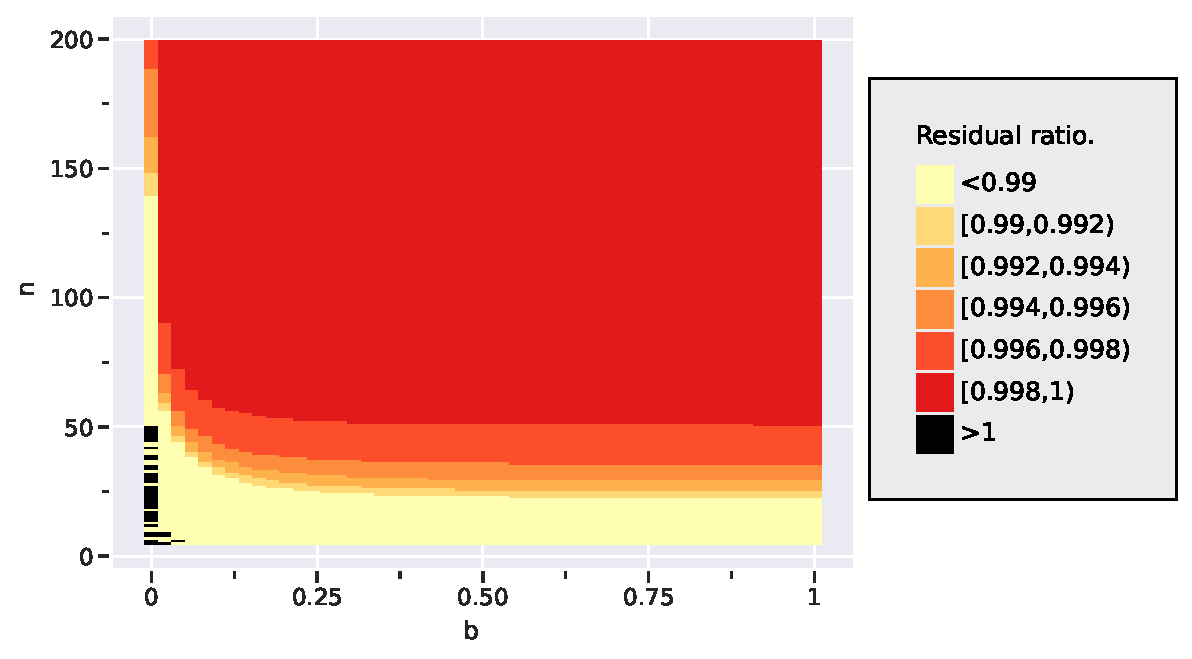
\includegraphics[width=\textwidth,height=2.08333in]{images/learned_policy_100.pdf}

}

\caption{\label{fig-learned\_policy\_b}\(\rho_{100}\). Note the
divergence in black, for low values of \(b\).}

\end{figure}%

\begin{figure}

\begin{minipage}{\linewidth}

\centering{

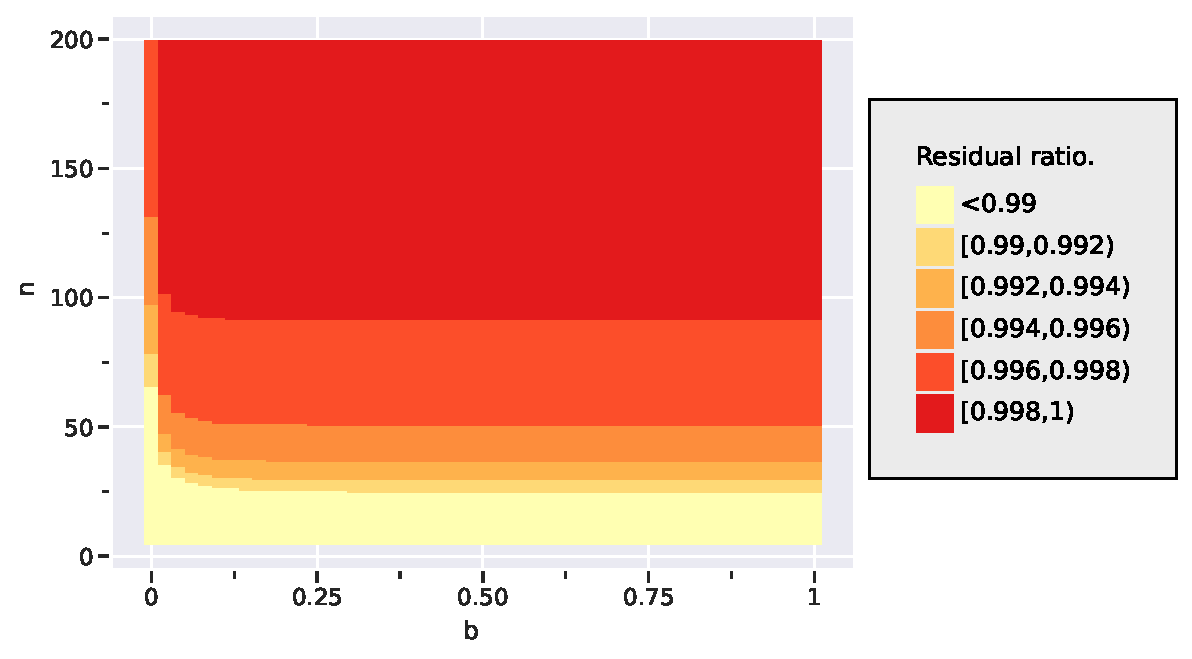
\includegraphics{images/learned_policy_10.pdf}

}

\subcaption{\label{fig-learned\_policy\_a}\(\rho_{10}\). Maximum
residual ratio: 0.99922.}

\end{minipage}%
\newline
\begin{minipage}{\linewidth}

\centering{

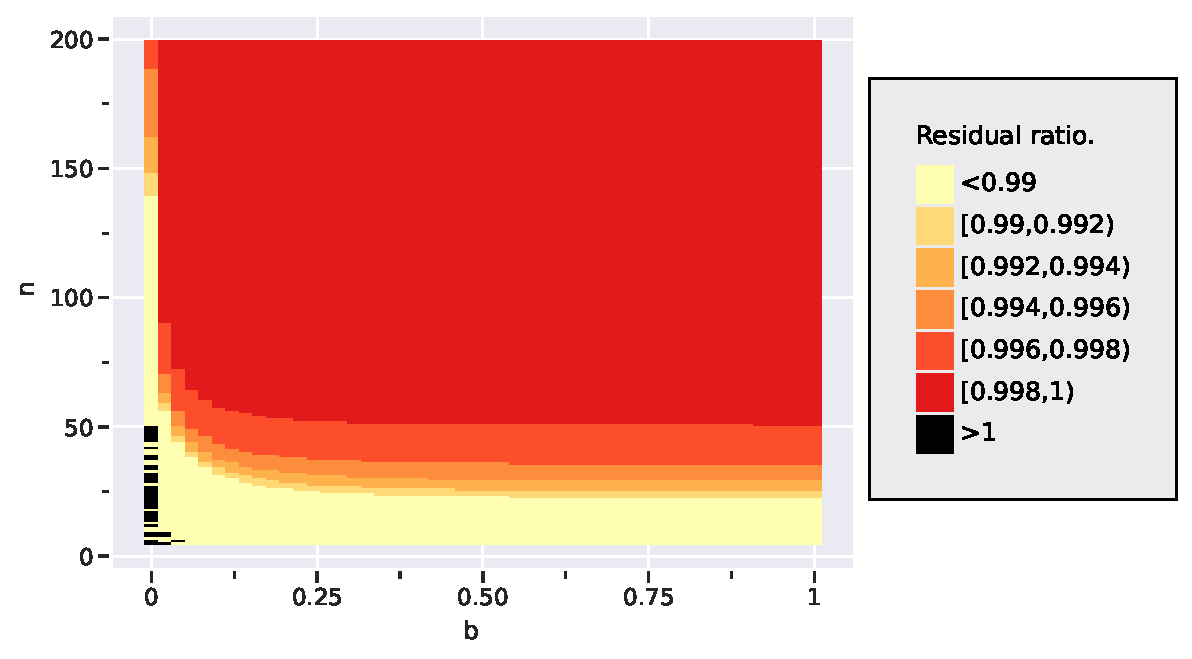
\includegraphics[width=\textwidth,height=2.08333in]{images/learned_policy_100.pdf}

}

\subcaption{\label{fig-learned\_policy\_b}\(\rho_{100}\). Note the
divergence in black, for low values of \(b\).}

\end{minipage}%

\caption{\label{fig-learned_policy}Evolution of the residual ratio
\(\rho_{10}\) and \(\rho_{100}\), with the learned policy, depending on
the problem parameters \(n\) and \(b\).}

\end{figure}%

\bookmarksetup{startatroot}

\chapter{Summary and Discussion}\label{summary-and-discussion}

In this thesis, we started with the idea of using numerical differential
equations solver as an iterative solver for a linear system. More
specifically, we turned our attention to a specific RK method, which has
two parameters to chose from, which we called the solver parameters. We
also chose a specific type of linear equation which arises from the
discretization of the steady state, one dimensional convection-diffusion
equation. This linear equation depends on two parameters, which we
called the problem parameters. The goal was then to see if we could
optimize for the solver parameters, as a function of the problem
parameters, to maximize the convergence rate of the method. To do that,
we used reinforcement learning. In particular, we applied the classical
REINFORCE algorithm to our problem. Using the implementation in this
thesis, we observed that the implemented solution works, with limited
results. In particular, if we use the parameter that we learn, it is
possible for the solver to diverge for some problem parameters. There
are some avenues to improve these results, in particular:

\begin{itemize}
\tightlist
\item
  On the technical front, the implemented algorithm is very elementary,
  and suffers from the issue of high sample variance, being a Monte
  Carlo method. This issue can be addressed by more better algorithms.
\item
  The policy used was a linear function of the problem parameters. We
  may want to explore if choosing a policy taking into account
  interactions between the problem parameters, or applying some
  transforms to them before fitting a linear policy. It is also possible
  to fit a neural network to the policy.
\item
  Possible incremental improvements can also be made. This involves for
  example experimenting with the reward function design, or setting a
  decaying learning rate to improve convergence of the RL algorithm.
\end{itemize}

At last, we need not restrict ourselves to just one type of solver. We
could potentially train an intelligent agent to chose which numerical
solver to use, depending on the problem.

There is on the other hand one glaring issue with the way that
reinforcement learning was applied to this problem. A core philosophy of
reinforcement learning is that the states, actions and rewards are all
interdependent. This interdependence was absent in this thesis, with the
state transition being random, no matter the action taken. While it was
possible to adapt this philosophy as presented in this thesis, this
somewhat hampers the utility of using reinforcement learning over other
methods. In particular, one may wonder if the implementation presented
here is essentially ``gradient descent, with extra steps''.

It is therefore preferable to change how the problem is approached. One
approach could be train an agent to dynamically change the solver
parameters over successive iterations for some specific set of
parameters. In that case, the agent would need information about the
evolution of the residual, which complicates the modeling problem.
Another approach would be to make use of meta learning {[}25{]}, where
instead of directly finding the optimal solver parameters, we learn how
to find them efficiently.

\bookmarksetup{startatroot}

\chapter*{References}\label{references}
\addcontentsline{toc}{chapter}{References}

\markboth{References}{References}

\phantomsection\label{refs}
\begin{CSLReferences}{0}{0}
\bibitem[\citeproctext]{ref-rombach2022highresolution}
\CSLLeftMargin{{[}1{]} }%
\CSLRightInline{R. Rombach, A. Blattmann, D. Lorenz, P. Esser, and B.
Ommer, {``High-resolution image synthesis with latent diffusion
models.''} 2022. Available: \url{https://arxiv.org/abs/2112.10752}}

\bibitem[\citeproctext]{ref-RL_robotics}
\CSLLeftMargin{{[}2{]} }%
\CSLRightInline{J. Kober, J. Bagnell, and J. Peters, {``Reinforcement
learning in robotics: A survey,''} \emph{The International Journal of
Robotics Research}, vol. 32, pp. 1238--1274, Sep. 2013, doi:
\href{https://doi.org/10.1177/0278364913495721}{10.1177/0278364913495721}.}

\bibitem[\citeproctext]{ref-RL_finance_review}
\CSLLeftMargin{{[}3{]} }%
\CSLRightInline{B. Hambly, R. Xu, and H. Yang, {``Recent advances in
reinforcement learning in finance,''} \emph{Mathematical Finance}, vol.
n/a, no. n/a, doi: \url{https://doi.org/10.1111/mafi.12382}.}

\bibitem[\citeproctext]{ref-chen2021survey}
\CSLLeftMargin{{[}4{]} }%
\CSLRightInline{X. Chen, L. Yao, J. McAuley, G. Zhou, and X. Wang, {``A
survey of deep reinforcement learning in recommender systems: A
systematic review and future directions.''} 2021. Available:
\url{https://arxiv.org/abs/2109.03540}}

\bibitem[\citeproctext]{ref-Silver2016}
\CSLLeftMargin{{[}5{]} }%
\CSLRightInline{D. Silver \emph{et al.}, {``Mastering the game of go
with deep neural networks and tree search,''} \emph{Nature}, vol. 529,
no. 7587, pp. 484--489, Jan. 2016, doi:
\href{https://doi.org/10.1038/nature16961}{10.1038/nature16961}.}

\bibitem[\citeproctext]{ref-Fawzi2022}
\CSLLeftMargin{{[}6{]} }%
\CSLRightInline{A. Fawzi \emph{et al.}, {``Discovering faster matrix
multiplication algorithms with reinforcement learning,''} \emph{Nature},
vol. 610, no. 7930, pp. 47--53, Oct. 2022, doi:
\href{https://doi.org/10.1038/s41586-022-05172-4}{10.1038/s41586-022-05172-4}.}

\bibitem[\citeproctext]{ref-cuomo2022scientific}
\CSLLeftMargin{{[}7{]} }%
\CSLRightInline{S. Cuomo, V. S. di Cola, F. Giampaolo, G. Rozza, M.
Raissi, and F. Piccialli, {``Scientific machine learning through
physics-informed neural networks: Where we are and what's next.''} 2022.
Available: \url{https://arxiv.org/abs/2201.05624}}

\bibitem[\citeproctext]{ref-Sutton1998}
\CSLLeftMargin{{[}8{]} }%
\CSLRightInline{R. S. Sutton and A. G. Barto, \emph{Reinforcement
learning: An introduction}, Second. The MIT Press, 2018. Available:
\url{http://incompleteideas.net/book/the-book-2nd.html}}

\bibitem[\citeproctext]{ref-towardsdatascienceReinforcementLearning}
\CSLLeftMargin{{[}9{]} }%
\CSLRightInline{C. Mahoney, {``Reinforcement learning: A review of the
historic, modern, and future applications of this special form of
machine learning.''}
\url{https://towardsdatascience.com/reinforcement-learning-fda8ff535bb6},
2021.}

\bibitem[\citeproctext]{ref-Williams1992}
\CSLLeftMargin{{[}10{]} }%
\CSLRightInline{R. J. Williams, {``Simple statistical gradient-following
algorithms for connectionist reinforcement learning,''} \emph{Machine
Learning}, vol. 8, no. 3, pp. 229--256, May 1992, doi:
\href{https://doi.org/10.1007/BF00992696}{10.1007/BF00992696}.}

\bibitem[\citeproctext]{ref-ODE_book}
\CSLLeftMargin{{[}11{]} }%
\CSLRightInline{W. A. Adkins, M. G. Davidson, and S. (Online service),
\emph{Ordinary differential equations}. in Undergraduate texts in
mathematics,. New York, NY : Springer New York :, 2012. Available:
\url{http://dx.doi.org/10.1007/978-1-4614-3618-8}}

\bibitem[\citeproctext]{ref-BellmanStab}
\CSLLeftMargin{{[}12{]} }%
\CSLRightInline{Bellman Richard Ernest, \emph{Stability theory of
differential equations /}. New York : McGraw-Hill, 1953.}

\bibitem[\citeproctext]{ref-convection_diffusion_book}
\CSLLeftMargin{{[}13{]} }%
\CSLRightInline{A. Atangana, \emph{Fractional operators with constant
and variable order with application to geo-hydrology}. Academic Press,
2018. Available:
\url{https://ludwig.lub.lu.se/login?url=https://www.sciencedirect.com/science/book/9780128096703}}

\bibitem[\citeproctext]{ref-NumDiffEqBook}
\CSLLeftMargin{{[}14{]} }%
\CSLRightInline{A. Iserles, \emph{A first course in the numerical
analysis of differential equations /}, 2. ed. in Cambridge texts in
applied mathematics. Cambridge ; Cambridge University Press, 2009.}

\bibitem[\citeproctext]{ref-BirkenNotes}
\CSLLeftMargin{{[}15{]} }%
\CSLRightInline{P. Birken, {``Numerical methods for stiff problems.''}
Lecture Notes, 2022.}

\bibitem[\citeproctext]{ref-iterative_method_book}
\CSLLeftMargin{{[}16{]} }%
\CSLRightInline{Wolfgang. Hackbusch and S. (Online service),
\emph{Iterative solution of large sparse systems of equations /}, 2nd
ed. 2016. in Applied mathematical sciences,. Cham : Springer
International Publishing :, 2016. Available:
\url{http://dx.doi.org/10.1007/978-3-319-28483-5}}

\bibitem[\citeproctext]{ref-NLA_book}
\CSLLeftMargin{{[}17{]} }%
\CSLRightInline{L. N. Trefethen and D. Bau, \emph{Numerical linear
algebra /}. Philadelphia : SIAM, Society for Industrial; Applied
Mathematics, cop. 1997.}

\bibitem[\citeproctext]{ref-aPrimerBrain}
\CSLLeftMargin{{[}18{]} }%
\CSLRightInline{E. Ludvig, M. Bellemare, and K. Pearson, {``A primer on
reinforcement learning in the brain: Psychological, computational, and
neural perspectives,''} in \emph{Computational Neuroscience for
Advancing Artificial Intelligence: Models, Methods and Applications},
2011, pp. 111--144. doi:
\href{https://doi.org/10.4018/978-1-60960-021-1.ch006}{10.4018/978-1-60960-021-1.ch006}.}

\bibitem[\citeproctext]{ref-reinforcementBookShiyuZhao}
\CSLLeftMargin{{[}19{]} }%
\CSLRightInline{S. Zhao, {``Mathematical foundations of reinforcement
learning.''} 2023.
\url{https://github.com/MathFoundationRL/Book-Mathmatical-Foundation-of-Reinforcement-Learning}
(accessed Mar. 30, 2023).}

\bibitem[\citeproctext]{ref-bellman1957dynamic}
\CSLLeftMargin{{[}20{]} }%
\CSLRightInline{R. Bellman, R. E. Bellman, and R. Corporation,
\emph{Dynamic programming}. in Rand corporation research study.
Princeton University Press, 1957. Available:
\url{https://books.google.se/books?id=rZW4ugAACAAJ}}

\bibitem[\citeproctext]{ref-trompCountingLegal}
\CSLLeftMargin{{[}21{]} }%
\CSLRightInline{J. Tromp, {``Counting legal positions in go ---
tromp.github.io.''} \url{https://tromp.github.io/go/legal.html}.}

\bibitem[\citeproctext]{ref-ross2007second}
\CSLLeftMargin{{[}22{]} }%
\CSLRightInline{S. M. Ross and E. A. Peköz, \emph{A second course in
probability}. ProbabilityBookstore.com, 2007. Available:
\url{https://books.google.se/books?id=g5j6DwAAQBAJ}}

\bibitem[\citeproctext]{ref-lillicrap2019continuous}
\CSLLeftMargin{{[}23{]} }%
\CSLRightInline{T. P. Lillicrap \emph{et al.}, {``Continuous control
with deep reinforcement learning.''} 2019. Available:
\url{https://arxiv.org/abs/1509.02971}}

\bibitem[\citeproctext]{ref-DBLP:journalsux2fcorrux2fSchulmanWDRK17}
\CSLLeftMargin{{[}24{]} }%
\CSLRightInline{J. Schulman, F. Wolski, P. Dhariwal, A. Radford, and O.
Klimov, {``Proximal policy optimization algorithms,''} \emph{CoRR}, vol.
abs/1707.06347, 2017, Available: \url{http://arxiv.org/abs/1707.06347}}

\bibitem[\citeproctext]{ref-gradient_descent_gradient_descent}
\CSLLeftMargin{{[}25{]} }%
\CSLRightInline{M. Andrychowicz \emph{et al.}, {``Learning to learn by
gradient descent by gradient descent,''} \emph{CoRR}, vol.
abs/1606.04474, 2016, Available: \url{http://arxiv.org/abs/1606.04474}}

\end{CSLReferences}



\end{document}
